\chapter{\IfLanguageName{dutch}{Stand van zaken}{State of the art}}
\label{ch:stand-van-zaken}
\graphicspath{{../../Images/}} 
% Tip: Begin elk hoofdstuk met een paragraaf inleiding die beschrijft hoe
% dit hoofdstuk past binnen het geheel van de bachelorproef. Geef in het
% bijzonder aan wat de link is met het vorige en volgende hoofdstuk.

% Pas na deze inleidende paragraaf komt de eerste sectiehoofding.

%%Dit hoofdstuk bevat je literatuurstudie. De inhoud gaat verder op de inleiding, maar zal het onderwerp van de bachelorproef *diepgaand* uitspitten. De bedoeling is dat de lezer na lezing van dit hoofdstuk helemaal op de hoogte is van de huidige stand van zaken (state-of-the-art) in het onderzoeksdomein. Iemand die niet vertrouwd is met het onderwerp, weet nu voldoende om de rest van het verhaal te kunnen volgen, zonder dat die er nog andere informatie moet over opzoeken \autocite{Pollefliet2011}.

%%Je verwijst bij elke bewering die je doet, vakterm die je introduceert, enz. naar je bronnen. In \LaTeX{} kan dat met het commando \texttt{$\backslash${textcite\{\}}} of \texttt{$\backslash${autocite\{\}}}. Als argument van het commando geef je de ``sleutel'' van een ``record'' in een bibliografische databank in het Bib\LaTeX{}-formaat (een tekstbestand). Als je expliciet naar de auteur verwijst in de zin, gebruik je \texttt{$\backslash${}textcite\{\}}.
%%Soms wil je de auteur niet expliciet vernoemen, dan gebruik je \texttt{$\backslash${}autocite\{\}}. In de volgende paragraaf een voorbeeld van elk.

%%\textcite{Knuth1998} schreef een van de standaardwerken over sorteer- en zoekalgoritmen. Experten zijn het erover eens dat cloud computing een interessante opportuniteit vormen, zowel voor gebruikers als voor dienstverleners op vlak van informatietechnologie~\autocite{Creeger2009}.
%\newpage
\section{Versiebeheer}
\subsection{Inleiding: De drie types van versiebeheersystemen}
\label{sec:vb_inleiding}
Versiebeheer is een belangrijk concept binnen softwareontwikkeling. Zo waren er in 2018 in het  totaal 100 miljoen projecten op het populaire versiebeheer platform GitHub \autocite{Git2018}. GitHub (sinds 2018 overgenomen door Microsoft) is niet de enige speler op de markt. Er zijn ook nog Code Commit van Amazon en GitLab. Veel bedrijven spelen dus in op de behoefte aan een duidelijk en efficiënt versiebeheersysteem. De vraag stelt zich dan ook: welke behoefte lossen deze systemen op?

Neem volgende scenario: Alice en Bob zijn aangenomen om te werken voor bedrijf X. Hun eerste taak is een website ontwikkelen. Ze leggen samen alle vereisten vast, bespreken de verschillende technologieën en gaan aan de slag. Op het einde van de eerste dag hebben ze elk een verschillende pagina gemaakt die ze graag met elkaar delen willen delen. Dit kan bijvoorbeeld door via mail de bestanden door te sturen. Een andere mogelijkheid is de bestanden via fysieke hardware zoals een USB-Stick aan elkaar te geven. Het nadeel is dat de code op twee verschillende plaatsen verspreid zit. Als Bob de code kwijt raakt, dan zal deze opnieuw moet worden geschreven. Om dit probleem te voorkomen kan men het project op een centrale server opslaan. Bob en Alice zullen hun veranderingen opslaan op deze centrale server. Zo hebben ze altijd toegang tot elkaars werk. 

Deze manier van werken heeft nadelen. Alice kan per ongeluk een bestand overschrijven of een stuk code verwijderen. Tenzij er back-ups zijn, is het originele bestand verloren. Om dit probleem te omzeilen, wordt er gebruik gemaakt van het concept van \textbf{versies}. Elke aanpassing die er gemaakt wordt resulteert in een nieuwe versie van het project. Men kan altijd terugkeren naar een eerdere versie. Als Alice dus het stukje code verwijdert in versie 15 kan men terug naar versie 14.

\textcite{Loeliger2009} stelt dat een versiebeheersysteem een middel is om verschillende versies van code te beheren en bij te houden. De auteur onderscheidt volgende drie eigenschappen waaraan dergelijke systemen voldoen:

\begin{itemize}
	\item er wordt gebruik gemaakt van een centraal archief. Binnen dit archief worden alle versies van het project bewaard en bijgewerkt.
	\item het centraal archief geeft toegang tot eerdere versies van het project.
	\item alle veranderingen die worden aangebracht aan het archief worden genoteerd in een centraal logboek.
\end{itemize}

Versiebeheer is geen nieuw concept. Er zijn zoals eerder aangehaald verschillende software oplossingen beschikbaar. Volgens \textcite{Chacon2014} zijn er drie grote categorieën (zie \ref{fig_types_cvs} voor een grafische weergave):

\begin{itemize}
	\item lokale versiebeheersystemen: het centraal archief waar de veranderingen in worden bewaard, staat op een lokale computer. Het grootste voordeel is dat een lokaal systeem zeer makkelijk te onderhouden is en eenvoudig op te stellen. Toch is het niet geschikt om bestanden met elkaar te  delen of samen aan bestanden te werken. Een gekend voorbeeld is RCS (Revision Control System) - zie \ref{sec:RCS} -. \\
	
	\item CVCS: om samen te kunnen werken aan dezelfde bestanden kan een CVCS (Centralised Version Control System) worden gebruikt. In plaats van het archief lokaal bij te houden wordt er gebruik gemaakt van een centrale server. Bestanden worden vervolgens lokaal gekopieerd. Als er veranderingen worden aangebracht zullen deze worden doorgestuurd naar de server.Doordat men verplicht is om de bestanden op een centrale plaats af te halen, kan men deze afschermen. Zo kan men de toegang beperken tot enkel de nodige bestanden per gebruiker. \\
	
Een neveneffect van alles centraal te beheren is het zogenaamde \textit{single point of failure (SPOF)} probleem. Een SPOF is een onderdeel van een systeem dat mocht het uitvallen heel het systeem tot een halt roept. Met andere woorden: valt het centraal archief weg heeft niemand nog toegang tot het project. Een mogelijke oplossing voor dit probleem is redundantie. Dit betekent het aanbieden van kopieën. \autocite{Sun2007}\\

	\item DVCS: om het SPOF probleem te voorkomen kan men kopieën maken van het centraal archief. Deze kopieën kunnen vervolgens worden verspreid over verschillende computers. Dit is het uitgangspunt van DVCS (Distributed version control System). Elke gebruiker heeft een lokale kopie van de centrale server. De veranderingen aan de bestanden worden eerst aangebracht in het lokaal archief en vervolgens gesynchroniseerd met de centrale variant.\\

Mocht het centraal aanspreekpunt niet beschikbaar zijn is dit geen probleem. Elke gebruiker heeft immers een volledige back-up van het volledige project. In theorie kan de gebruiker zelfs optreden als nieuwe centrale server.
\end{itemize}


\begin{figure}[h!]
	\centering
	\begin{subfigure}[b]{.5\textwidth}
	\centering
		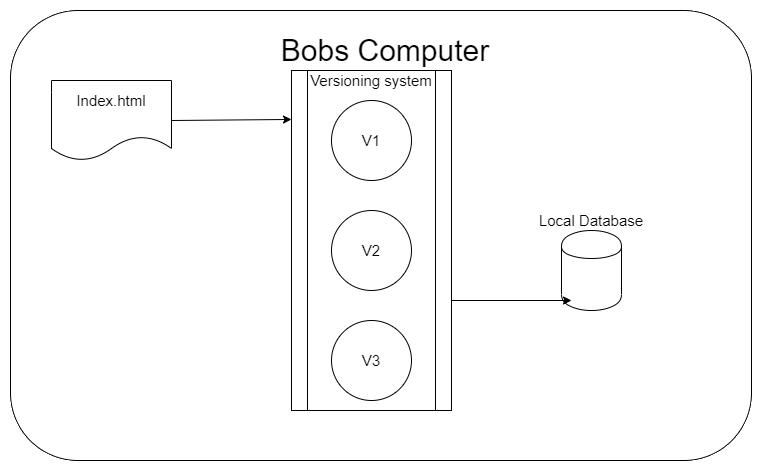
\includegraphics[scale=.3]{LVCS.png}
		\caption[Overzicht structuur Lokale VCS]{Overzicht van de structuur van een Lokale VCS.}
	\end{subfigure}%
	\begin{subfigure}[b]{.5\textwidth}
	\centering
		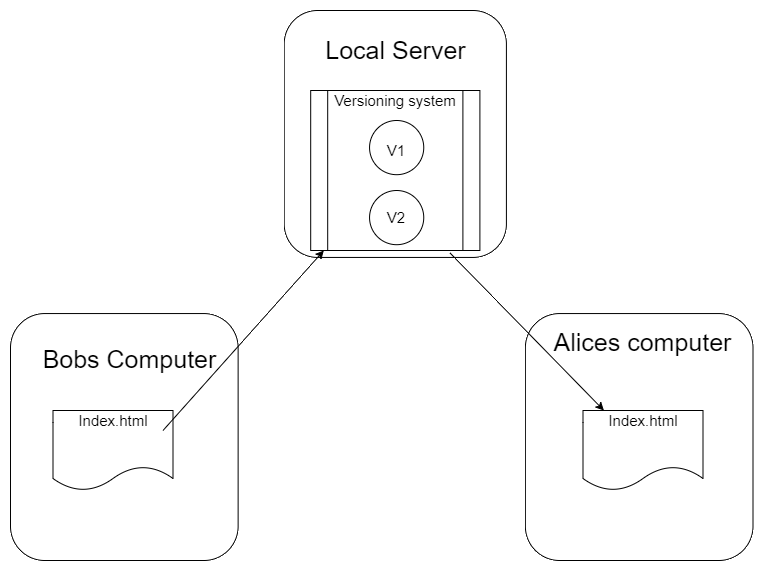
\includegraphics[scale=.3]{CVCS.png}
			\caption[Overzicht structuur CVCS]{Overzicht van de structuur van een CVCS.}
	\end{subfigure}%
	\hfill
	\begin{subfigure}{.5\textwidth}
		\centering
		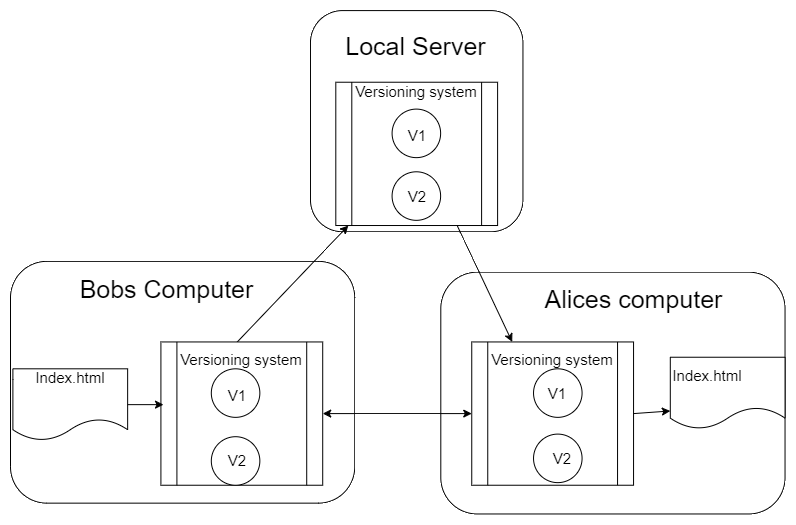
\includegraphics[scale=0.3]{DVCS.png}
	\caption[Overzicht structuur DVCS]{Overzicht van de structuur van een DVCS.}
	\end{subfigure}
	
	\caption[Overzicht types VCS]{Overzicht van de drie types van VCS zoals aangegeven door \textcite{Chacon2014}.}\label{fig_types_cvs}
\end{figure}

	
\subsection{RCS: één van de eerste lokale versiebeheersystemen.}
\label{sec:RCS}


RCS \textit{(Revision Control System)} is een lokaal versiebeheer systeem. Het wordt voor het eerst beschreven in een artikel geschreven door \textcite{Tichy85rcs}. Het werd verder ontwikkeld binnen het GNU project -Een open source besturingssysteem \footnote{GNU is veel meer dan enkel open source. Het GNU project is sterk verbonden met de ideologie en organisatie van de free software foundation (FSF). Meer informatie omtrent deze organisatie en beweging is te vinden op: \url{https://www.fsf.org/}}- waar het als vervanging voor het CSSC Systeem \autocite{GNUCSSC} werd gebruikt. CSSC is een systeem gebaseerd op SCCS (Source code control system) dat ontworpen is voor UNIX systemen. SCCS is in opdracht van Bell Labs ontwikkeld door \textcite{Rochkind1975}.\\

Voordat RCS op de markt kwam is er nog tal van andere software ontwikkeld. Zo was er CA-Panvalet een gepatenteerde oplossing voor Mainframe computers.\\

Waarom is het interessanter om RCS in detail te bekijken? Veel van de concepten waar het gebruik van maakt zijn aanwezig in moderne systemen (zoals GIT). Het is open source en wordt nog steeds op vrijwillige basis onderhouden, wat aansluit bij de visie van deze bachelorproef.\\

De manier waarop versies worden bijgehouden in RCS -zoals door \textcite{Tichy85rcs} beschreven- is gebaseerd op een boomstructuur -denk aan een stamboom-. Volgens \textcite{Lievens2019}, is een boom een collectie van \textbf{toppen} \textit{(in het Engels ook wel Nodes genoemd)}. Deze toppen hebben een hiërarchische verband.Zo bestaat er bijvoorbeeld een kind-ouder verband. Er zijn twee bijzondere toppen in een boom:

\begin{itemize}
	\item de wortel(\textit{root}): Deze top ligt helemaal aan het begin van de boom. Alle andere toppen zijn afstammelingen van deze top. Het heeft aldus geen ouders.
	\item een blad(\textit{leaf}): Deze top heeft geen kinderen. In tegenstelling tot een wortel kunnen er meerdere bladeren aanwezig zijn.
\end{itemize}

Alle andere toppen worden intermediair genoemd. Elke top heeft mogelijk een aantal kinderen. De diepte van de wortel is nul ($d$=1) en elk kind heeft als diepte: 

\begin{equation}
	d_{kind} = d_{ouder} + 1
\end{equation}

Elk van deze kinderen is op zijn beurt de wortel voor een nieuwe deelboom. Het concept van \textbf{diepte} is belangrijk. 

Al deze concepten worden ook nog eens grafisch verduidelijkt in de figuur \ref{fig_tree}.

\begin{figure}[h!]
\centering
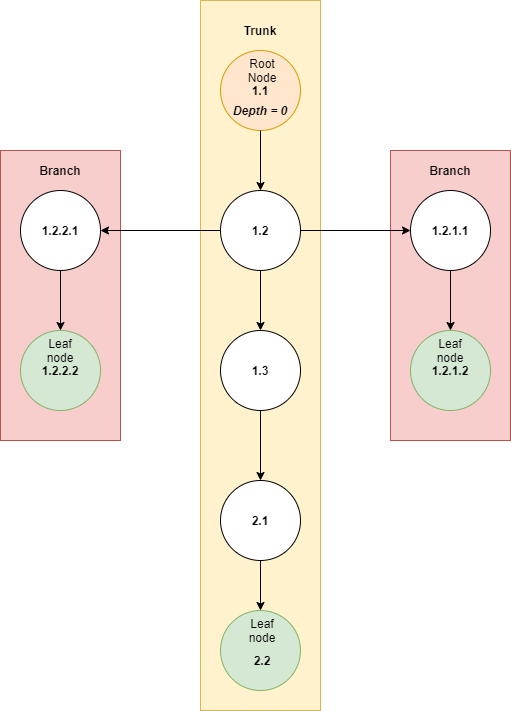
\includegraphics[scale=0.5]{tree1.png}
\caption[Overzicht concepten boomstructuur]{Een overzicht van alle concepten binnen een boomstructuur waar RCS van gebruik maakt.}\label{fig_tree}
\end{figure}

Er kan gebruik gemaakt worden van een boomstructuur om de onderlinge relaties tussen de versies weer te geven. Stel: Bob en Alice zijn bezig aan de hoofdpagina. Bob maakt een initiële versie van de pagina. Vervolgens wilt hij die graag delen met Alice. Hiervoor gebruikt hij het commando om een nieuwe versie aan te maken: \Verb+ci homepage.html+. Dit commando wordt \textbf{inchecken} genoemd. Binnen GIT is dit vergelijkbaar met het commando \textit{git push}. Aangezien dit de eerste versie is kan men dit vergelijken met het aanmaken van een wortel. Volgende versies worden kinderen van de vorige versie. Zo wordt versie 1.4 kind van versie 1.3. Inchecken gaat niet alleen onze boomstructuur aanmaken maar ook de extensie \textit{.v} toevoegen (\verb+homepage.html.v+). Het originele bestand wordt ook verwijderd\\

Het bestand krijgt ook een \textbf{versienummer}. Dit versienummer heeft de vorm: $x_1.x_2$.\ $x_1$ (ook wel \textit{release} genoemd) staat voor een grote verandering. Bijvoorbeeld het in productie nemen van een nieuwe versie.$x_2$ (\textit{level}) staat voor een kleinere verandering. Een andere manier om $x_2$ te bekijken is de diepte met als wortel de laatste release ($x_1$). 1.1 is het versienummer van de wortel die Bob heeft aangemaakt. 1.4 is het derde kind van de wortel.Elke check-in zal het level ($x_2$) met één verhogen. Het release nummer ($x_1$) wordt manueel verhoogd door middel van de \textit{-r} optie bij check-in \footnote{\Verb+ci -r2 homepage.html+}. Bij branches is er ook nog spraken van $x_3$ en $x_4$ zie \ref{par:branches}.\\

Deze manier van versies te bestempelen wordt nog steeds gebruikt. Het is echter niet de enige manier. \textit{Semantic versioning} is een gekend alternatief. Het concept van versienummers bestaat in Git onder de vorm van \textit{tags}.\\

Er is nu een bestand onder de vorm \verb+homepage.html.v+. Hoe kan Alice nu dit bestand aanpassen en een nieuwe versie publiceren? Alice zal het bestand moeten \textbf{uitchecken}.Dit kan ze doen door middel van het commando \verb+co+ en de naam van het bestand \footnote{(\Verb+co homepage.html+)} . Het uitchecken is aldus het verkrijgen van een specifieke versie uit het archief. Als er geen specifieke versie wordt meegegeven wordt de laatste versie opgehaald. Om een specifieke versie op te halen kan er gebruik gemaakt worden van de optie -r  \footnote{(\Verb+co -r1.1 homepage.html+)} . Alice heeft nu een kopie van het originele bestand gekregen. Merk op dat in tegenstelling tot inchecken ons archief niet wordt verwijderd. Vervolgens kan ze in deze lokale kopie wijzigingen aanbrengen. Tot slot wordt het bestand weer aan het lokaal archief toegevoegd door middel van inchecken. Het equivalent van \verb+co+ binnen git is \verb+git pull+.\\

\begin{wrapfigure}{r}{0.5\textwidth}
\begin{center}
  	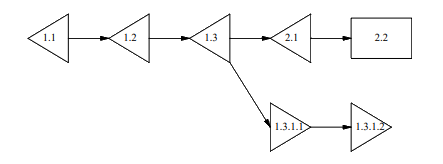
\includegraphics[scale=0.6]{deltas.png}
\end{center}
\caption[Voorbeeld van deltas.]{Een voorbeeld van deltas.De Trunk bevat een series van achterwaardse deltas terwijl alle branches enkel voorwaardse deltas bevatten. Grafiek afkomstig uit \textcite{Tichy85rcs}}\label{fig_deltas}
\end{wrapfigure}

Hoe worden de verschillen tussen de versies bijgehouden in ons lokaal archief? Een mogelijke oplossing zou zijn om alle versies van het bestand afzonderlijk bij te houden. Dit vraagt veel opslagruimte. RCS gebruikt voor dit probleem het concept van \textbf{deltas}. Een delta houdt bij welke regels veranderd zijn ten opzichte van de vorige versie. Doordat de delta enkel de relevante lijnen bijhoudt wordt de opslag beperkt \footnote{De delta wordt opgebouwd aan de hand van het GNU commando diff \url{https://www.gnu.org/software/diffutils/}}. Er zijn twee types van deltas: \textbf{voorwaartse deltas} en \textbf{achterwaartse deltas}. Bij het inchecken van een nieuwe versie zal de vorige versie worden vervangen door een achterwaartse delta. Zit men momenteel op versie 1.3 en  vraagt men versie 1.2 dan zal de achterwaardse delta van versie 1.2 worden toegepast op versie 1.3. (Voorwaardse deltas komen aan bod in het gedeelte over branching (\ref{par:branches}). Het concept van deltas wordt nog eens verduidelijkt door een voorbeeld in de appendix -zie \ref{ch:voorbeeld-rcs}-.)\\

Inchecken en uitchecken ligt aan de basis van het archiefsysteem. Toch is er nog een probleem aanwezig met deze manier van werken. Stel dat Alice en Bob gelijktijdig wijzigingen aanbrengen aan een bestand. Ze willen dit bestand elk afzonderlijk publiceren.  Hierdoor ontstaan er twee versies die afstammen van één gezamenlijke versie. De boomstructuur wordt in twee gesplitst. Dit is niet mogelijk aangezien een versie altijd uniek moet zijn. Hoe kan men verzekeren dat elke versie slechts één kind heeft (op dezelfde branch)? Dit probleem wordt opgelost door \textbf{sloten}(engels=lock).Dit concept geeft gebruikers de mogelijkheid om een versie te  versleutelen. Terwijl een versie versleuteld is kan niemand anders wijzigingen aanbrengen. Andere gebruikers kunnen deze nog bekijken. Op het moment dat Bob zijn versie gaat uitchecken kan hij deze versleutelen (door middel van de \textit{-l} optie bij het co commando). Hierdoor kan Alice geen nieuwe versie meer aanmaken tot Bob zijn wijzigingen heeft doorgevoerd. Met andere woorden zolang Bob het slot niet vrijgeeft kunnen er geen nieuwe versies worden aangemaakt\footnote{In sommige gevallen kan het slot ook worden 'geforceerd' mocht Bob bijvoorbeeld ziek vallen}. Deze manier van werken heeft een zichtbaar nadeel. Alice is verplicht om te wachten op Bobs nieuwe versie alvorens ze veranderingen kan aanbrengen. Git gebruikt het concept van sloten niet. Daar maakt men gebruik van \textbf{merges} om dit zelfde probleem aan te pakken %\ref{sec:GIT}%.

\subsubsection{Opmerkingen}
In het originele artikel wordt de klemtoon gelegd op het onderling delen van de verschillende versies. Hierdoor kan men de indruk krijgen dat er een centrale server betrokken is. Dit is niet het geval. De software is ontworpen om op één besturingssysteem uitgevoerd te worden. Volgens \textcite{Debian2020} is GNU aangezien het gebaseerd is op UNIX een \textit{multi-user os}. Dat wil zeggen dat meerdere gebruikers het systeem tezelfdertijd kunnen gebruiken door middel van een terminal connectie. Hierdoor kan men onderling de bestanden delen ondanks dat men niet gaat werken in een CVCS.

\subsection{branches}
\label{par:branches}
\subsubsection{Duiding}
Door het principe van sloten en inchecken lijkt het alsof elke versie exact één opvolger heeft. Zo zal versie 1.3 de opvolger zijn van 1.2. Toch kunnen er zich zoals in een stamboom  vertakkingen voordoen. De vertakkingen worden \textbf{Branches} genoemd. De hoofdboom (niet vertakte toppen die afstammen van de wortel) wordt de \textbf{trunk} genoemd. Dit principe kan men het best demonstreren aan de hand van een figuur. Zo kan men zien in figuur \ref{fig_tree} dat er twee vertakkingen zijn op versie 1.2. Het principe van vertakkingen lijkt op het eerste zicht complex en onoverzichtelijk. \textcite{Tichy85rcs} geeft enkele redenen om dit toch toe te passen.

\begin{enumerate}
\item Doorvoeren van veranderingen in oude versies: Stel dat een bedrijf een oude versie van een software product gebruikt. Dit product is ontwikkeld met behulp van RCS. Er wordt een fout in deze oude versie gevonden die om een oplossing vraagt. Aangezien er in de tussentijd nieuwere versies zijn is dit niet evident. Het bedrijf zou volledig moeten overstappen op de nieuwste versie alvorens een aanpassing kan gebeuren. Om deze situatie te vermijden kan men gebruik maken van vertakkingen. Zo kan men een vertakking maken op de gewenste versie en kleine aanpassingen doorvoeren.\\
\item Andere implementaties: stel dat een ontwikkelaar een nieuw stuk code wilt uittesten. Deze heeft niet het gewenste resultaat. Mocht dit stuk code bewaard worden op de hoofdboom (\textit{trunk}) dan is er een onstabiele versie gepubliceerd. Een gebruiker die op dat moment de recentste versie opvraagt, krijgt dus een niet werkend product.\\
Door branches te gebruiken kan men ervoor zorgen dat er enkel werkende versie op de hoofdboom terecht komen. Nieuwe stukken code worden eerst geïsoleerd en getest alvorens opgenomen te worden. Op die manier blijft het archief in een overzichtelijke en stabiele vorm.
\end{enumerate}

\begin{wrapfigure}{L}{0.5\textwidth}
\begin{center}
  	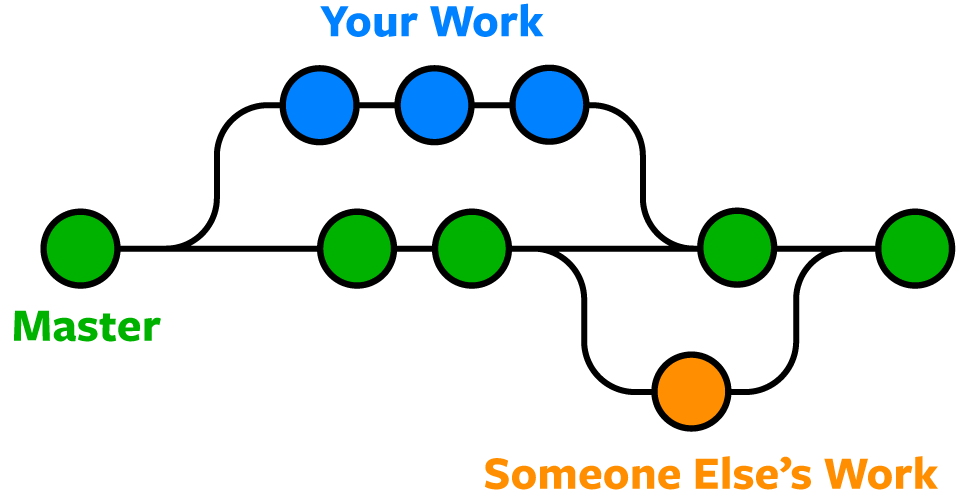
\includegraphics[scale=0.2]{git-branches-merge.png}
\end{center}
\caption[Voorbeeld merge proces.]{Een voorbeeld van een merge proces. Eerst wordt er een branch aangemaakt die na drie versies terug in de master wordt gemerged. Grafiek gepubliceerd door \textcite{NobleDesktop2018}}\label{fig_merge}
\end{wrapfigure}

Door middel van vertakkingen kan code worden geschreven en de hoofdboom stabiel gehouden. Zelfs met veel ontwikkelaars en grote projecten kan men door deze manier van werken code conflicten vermijden. Eenmaal de code klaar is voor productie kan men deze gaan publiceren op de hoofdboom. Dit concept wordt ook wel \textbf{mergen} genoemd. Dit principe wordt geïllustreerd door de figuur \ref{fig_merge}.

%todo uitleg van RCS branching en forward deltas

\subsubsection{Flows}
Er is echter nog een grote vraag die niet beantwoord is: wanneer moet men gaan vertakken?

De eerste reden aangehaald door \textcite{Tichy85rcs} -het doorvoeren van veranderingen- is minder relevant binnen de context van DVCS. Er wordt namelijk niet meer op een gezamenlijk archief gewerkt maar op een lokale kopie. Het bedrijf kan dus op zijn eigen kopie lokaal veranderingen aanbrengen .De tweede reden is echter wel belangrijk. Stel dat een project honderden bestanden en ontwikkelaars heeft. In zo een omgeving kunnen veranderingen soms onvoorspelbare gevolgen hebben. Ontwikkelaars kunnen het project vertakken, wijzigen en testen alvorens het in productie te nemen. Dit is het principe achter \textbf{feature branches}.\\

%Voeg meer bron vermeldingen toe

Bij grote software projecten loopt men het risico dat er veel aftakkingen worden gemaakt die niet worden gebruikt (\textbf{branchmania}). Het artikel van \textcite{Bird2012}, benadrukt het belang van levende takken. Dit zijn vertakkingen die actief wordt gebruikt. Dit kan enkel bereikt worden via een duidelijke werkwijze. Deze werkwijze om het aantal vertakkingen zo klein mogelijk te houden wordt geïllustreerd in figuur \ref{fig_mic_flow}.

\begin{figure}
\begin{center}
  	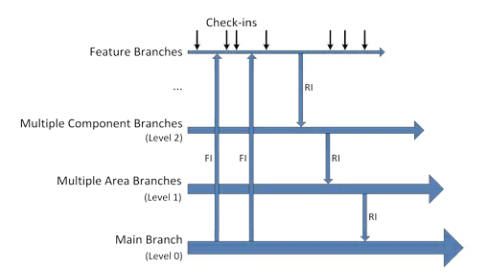
\includegraphics[scale=1]{microsoft-branching.png}
\end{center}
\caption[Voorbeeld flow]{Flow zoals vermeld in het artikel van  \textcite{Bird2012}}\label{fig_mic_flow}
\end{figure}

Elke ontwikkelaar schrijft zijn code op een feature branch. Het risico hiervan is dat men op den duur niet meer compatibel is met de hoofdboom. Er kunnen sinds de vertakking immers verschillende andere versies gepubliceerd zijn. Daarom wordt er  gewerkt met twee tussenbranches. Hier test men of de code compatibel is met de verschillende andere onderdelen van de software. Het proces waarbij men feature branches integreert in andere tussenbranches noemt men ook wel \textbf{Reverse integration} -aangeduid als RI op de figuur-. Een ander principe dat gebruikt wordt is dat van \textbf{Forward integration}. Hierbij worden de nieuwe versies van de hoofdbranch (ook wel master genoemd) geplaatst op de feature branch. Zo blijft de feature branch compatibel met alle veranderingen.



%\subsection{GIT}
%\label{sec:GIT}

\subsection{Conclusie}
\label{vb_conclusie}
De verschillende types van versiebeheersystemen -zoals besproken in \ref{sec:vb_inleiding}- hebben een gemeenschappelijke eigenschap. De bestanden en in veel gevallen het archief staan integraal opgeslagen op computers. Bij lokale versiebeheersystemen en CVCS staat het zelfs op één centrale computer. Dit introduceert het probleem van een SPOF (Single point of failure).DVCS vermijdt dit probleem door gebruikers kopieën te geven van het archief. Valt de centrale computer weg dan heeft elke gebruiker een back-up. Veranderingen tussen lokale versies en die op de centrale computer moet manueel gesynchroniseerd worden. Hierdoor heeft men in grote mate controle over wat er centraal wordt opgenomen. Het nadeel is dat er veel lokale kopieën zijn en veranderingen niet altijd worden gesynchroniseerd. Op deze manier heeft niet iedereen toegang tot de laatste veranderingen. Het zou dus een verbetering zijn mocht er een systeem bestaan dat één centraal archief ondersteunt zonder SPOF. Dit lijkt op eerste zicht niet mogelijk, aangezien er één centraal aanspreekpunt moet zijn. Toch is dit probleem al eerder opgelost onder de vorm van peer-to-peer (afgekort tot p2p) netwerken.\\

P2P is voornamelijk bekend onder de vorm van file-sharing netwerken zoals Napster. \textcite{Chawathe2003} stellen dat Napster één van de eerste systemen was die erin slaagde om een succesvol netwerk uit te bouwen. Bij dit netwerk worden files niet opgevraagd aan een centrale server. In plaats hiervan gebruikt men een netwerk van \textbf{peers}. Door de principes van dit type van netwerken toe te passen kan men een centraal archief op een gedistribueerde manier opslaan. Zo behoudt men het voordeel van CVCS zonder een SPOF. \\

De doelstelling van deze bachelorproef is om een werkend P2P versiebeheersysteem te gaan implementeren. Hiervoor moet men afbakenen welke functionaliteiten deze implementatie moet voorzien. In vorige paragrafen werden de verschillende concepten besproken. Hieronder volgt een oplijsting van deze verschillende concepten alsook een korte uitleg. Hierbij worden de terminologie en concepten van Git gebruikt. Deze worden vervolgens meegenomen naar volgende hoofdstukken, waar een implementatie wordt voorzien.

\begin{table}[h!]
	\centering
	\begin{tabular}{ |p{2cm}|p{12cm}|}
 		\hline
 		\multicolumn{2}{|c|}{\large \textbf{Concepten binnen versiebeheer}} \\
 		\hline
 		\textbf{Begrip}	& \textbf{Uitleg}\\
 		\hline
 		\textbf{Archief} & Een centrale plaats voor het bijhouden van bestanden. De wijzigingen van deze gearchiveerde bestanden worden bijgehouden. Men kan zowel historische als recente versies van het bestand opvragen alsook van het gehele archief.\\
 		\hline
 		\textbf{Versies} & Elke wijziging binnen het archief leidt tot een nieuwe versie. Men kan de verschillende versies ten alle tijden raadplegen. Men kan ook oudere versies gebruiken voor branching. In extreme gevallen kan een archief volledig worden teruggedraaid naar een eerdere versie.\\
 		\hline
		\textbf{Logboek} & Een bestand waarin alle wijzigingen worden bijgehouden. Het logboek is ook onderdeel van het archief. \\
		\hline
		Pushing	& Het principe waarbij wijzigingen die lokaal worden aangebracht, worden gesynchroniseerd met de centrale server.\\
		\hline
		Pulling & Het binnenhalen van veranderingen aangebracht op het centraal archief naar een lokale kopie.\\
		\hline
		Clonen & Het aanmaken van een lokale kopie van een centraal archief. \\
		Branching & Het voorzien van alternatieve vertakkingen van het archief. \\
		\hline
	\end{tabular}
	\label{tbl_concepts}
	\caption{Concepten binnen versiebeheersystemen.}
\end{table}
\newpage
\section{Het omspringen met bestanden in een gedecentraliseerd systeem}
\label{IPFS}
\subsection{Duiding van dit hoofdstuk}
\label{Duiding_IPFS}
De doelstelling van deze bachelorproef is om een volledig gedecentraliseerd versiebeheersysteem uit te werken. Zoals in de vorige sectie reeds werd uitgelegd is een versiebeheersysteem een verzameling van bestanden en een logboek waarin alle veranderingen aan deze bestanden worden bijgehouden. Dit logboek is aldus een collectie van data. Hierdoor kan een logboek eenvoudig worden gedecentraliseerd aan de hand van een blockchain. \textbf{Maar ook dan blijft de vraag nog steeds waar kunnen de bestanden worden bewaard?}\\

In eerste instantie lijkt het eenvoudig om deze bestanden ook gewoon op een blockchain te zetten. Dit is echter niet mogelijk (hier wordt verder op ingegaan in hoofdstuk 3). Een andere eenvoudige oplossing zou zijn dat Bob gewoon rechtstreeks de bestanden deelt met Alice. Dit kan doormidden van een FTP connectie of andere oplossingen. Hierdoor komen Bob en Alice echter in een klassiek server-client model terecht. De nadelen van dit model worden uitvoerig besproken in \ref{ipfs_decent}. Er is dus een manier nodig om bestanden te delen zonder dat men daarbij gebruik moet maken van een server. Dit principe wordt ook wel \textbf{gedecentraliseerde file-sharing} genoemd.\\

Dit probleem is niet nieuw. Er bestaan al reeds sinds de vroege jaren 2000 verschillende protocollen die dit probleem proberen oplossen. Doorheen dit hoofdstuk worden drie van deze protocollen besproken: Bit-Torrent, Gnutella en IPFS. Waarom wordt er juist geopteerd voor deze drie protocollen? Bit-Torrent en Gnutella zijn een mooi voorbeeld van twee verschillende types van protocollen. Bij Bit-Torrent is er namelijk nog spraken van een zekere mate van centralisatie -zie \ref{torrenting}-. Gnutella is volledig gedecentraliseerd maar heeft ook een aantal beperkingen -zie \ref{Gnutella}. Tot slot komen we tot een meer recent protocol dat veel van de beperkingen van de vorige twee protocollen opvangt. Dit protocol wordt IPFS genoemd en is het protocol dat wordt gebruikt in de POC. Deze protocollen vereisen wel enige voorkennis om te begrijpen. Daarom volgt er eerst een korte introductie van alle begrippen.
\subsection{Algemene begrippen en concepten}
\label{ipfs_decent}

\subsubsection{Decentraliseren en P2P}
Zoals in de vorige sectie uitgelegd moeten de bestanden worden opgeslagen op een gedecentraliseerd systeem. \textbf{Wat betekend het om iets te gaan decentraliseren?} Kort gesteld is een gedecentraliseerd systeem een systeem waar geen centrale component aanwezig is.\\

Een gekend voorbeeld van een gecentraliseerd systeem is de manier waarop mensen surfen op het internet. Stel onderstaand scenario:\\

Bob is een liefhebber van Capybaras en wil informatie krijgen over de dieren. Hij surft bijgevolg naar de Wikipedia pagina. Bob zal een verzoek moeten sturen naar de server van Wikipedia. Hiervoor moet hij het publieke IP-Adres kennen. Dit kan hij verkrijgen door het DNS protocol. Bob stuurt zijn verzoek naar deze server en krijgt de gezochte pagina terug. Aangezien alle informatie zich bevindt op één plaats kan er worden gesproken van een gecentraliseerd systeem. Dit specifiek type van een centraal systeem wordt ook wel een \textbf{client-server} systeem genoemd.\\

Binnen een gedecentraliseerd systeem is er geen spraken meer van een centrale server die alles ter beschikking stelt. Alle computers zijn onderling met elkaar verbonden en wisselen bestanden en gegevens met elkaar uit. Dit wordt ook wel bestempeld als \textbf{Peer-to-Peer}(afkort als P2P). Peer-to-peer is een vorm van distributed computing\footnote{\textbf{Distributed Computing}: een collectie van individuele computers die verbonden zitten in een netwerk en met elkaar kunnen communiceren. Deze computers zijn in staat om samen computermatige taken uit te voeren. (\autocite{Attiya2004})} waarbinnen elke computer optreedt als een Servent. Dit is een combinatie van het woord \textbf{ser}ver en cli\textbf{ent}. Elke computer op dit netwerk is aldus in staat om verzoeken te behandelen en te versturen. Het biedt met andere woorden een gangbaar alternatief voor het client-server model. \\
 
Volgens \textcite{Schollmeier2001} zijn er  twee verschillende categorieën van Peer-to-peer netwerken:

\begin{itemize}
\item Pure netwerken: hierbij is elke peer gelijkwaardig. Dat wilt zeggen dat iedere individuele deelnemer evenveel privileges en taken heeft. Kortom is één van die deelnemers niet meer bereikbaar dan kan elke andere peer zijn rol op zich nemen. Een voorbeeld van zo een netwerk is Gnutella.\\
\item Hybride netwerk: er is één centrale component aanwezig die een bepaalde taak op zich neemt. Bijvoorbeeld bij het Bit-Torrent protocol is er een centrale component nodig om toe te treden tot het netwerk. Als deze centrale component onbereikbaar is functioneert het netwerk niet.\\
\end{itemize}


\textbf{Waarom zouden we dus kiezen voor een gedecentraliseerd systeem?} Om dit duidelijk te maken kunnen de voor~ en nadelen worden samengevat in onderstaande tabel:\\

\begin{table}[h!]
	\centering
	\begin{tabular}{ |p{3cm}|p{6cm}|p{6cm}|}
		\hline
		\multicolumn{3}{|c|}{Vergelijking Gecentraliseerd en Gedecentraliseerd Systeem}\\
		\hline
		\textbf{Probleem}&\textbf{Client-Server}&\textbf{P2P}\\
		\hline
		\textbf{SPOF}&Doordat alle informatie zich op één server bevindt is er ook één kritieke plaats waar alles kan fout lopen. Is de server onbeschikbaar zijn alle diensten en informatie hierop dat ook.& Er is niet één computer die optreedt als server. Elke deelnemer van het netwerk (ook wel \textbf{Peer} genoemd) treedt op als server en cliënt. Waardoor er geen kritiek punt is waarop het kan fout lopen is.\footnote{Zoals hierboven vermeld geld dit enkel voor een puur netwerk. Een hybride netwerk heeft nog steeds het probleem van SPOF.}\\
		\hline
		\textbf{Netwerkbelasting}&Doordat al het verkeer moet verwerkt worden door dezelfde hardware kan dit leiden tot een hoge serverbelasting. Hierdoor kan het verwerken van deze verzoeken traag verlopen.&Het hele netwerk verwerkt onderling verzoeken waardoor de individuele belasting op één peer eerder laag blijft. Hierdoor is het netwerk instaat om op een efficiënte manier verzoeken te verwerken.\\
		\hline
		\textbf{Uitbreidbaarheid}&Het uitbreiden van bestaande infrastructuur is niet evident en vereist vaak grote kosten voor een bedrijf.&Een p2p netwerk is goed uitbreidbaar. Op elk moment kunnen computers toetreden tot het netwerk of uittreden.\\
		\hline
	\end{tabular}
	\label{tbl_concepts}
	\caption{Vergelijking tussen gecentraliseerd - gedecentraliseerd systeem}
\end{table}
\newpage
\subsubsection{Hashing}
\label{hashing}
Hashfuncties is een begrip dat veel aan bod komt in de verschillende protocollen.  Zeker binnen IPFS speelt hashing een grote rol. Daarom is het noodzakelijk dat het begrip toch kort wordt toegelicht.\\

Hashfuncties liggen aan de basis van het verifiëren van de dataintegriteit bij bestanden. Het is immers belangrijk om te kunnen nagaan of het bestand dat verkregen is hetzelfde is als wat verwacht wordt. Op deze manier kan er worden nagegaan of de bestanden eventueel beschadigd zijn door de overdracht. Een \textit{goede} hashfunctie zou moeten voldoen aan volgende eigenschappen (\autocite{Anderson93}):

\begin{itemize}
\item One-way functie: het is relatief eenvoudig om voor een gegeven dataset $x$ een resultaat te vinden $f(x)$. Het is echter onwaarschijnlijk om voor een gegeven resultaat $f(x)$ de originele dataset $x$ te vinden. Op deze manier is het makkelijk om een dataset te valideren indien de hashfunctie waarde gegeven.\\
\item Collision free: het moet niet mogelijk zijn dat twee verschillende datasets (bijvoorbeeld: $x$ en $y$) dezelfde hashfunctie waarde hebben. Wiskundig kan dit worden voorgesteld door volgende notatie: stel een functie $f:A->B$. Deze functie is collision free indien $\forall \{x,y\}|\{x,y\} \subseteq A | f(x) \neq f(y)$\\
\item Gelijke verdeling: een kleine verandering aan de dataset leidt tot een volledig verschillende hashwaarde. Zo is hashwaarde voor 123 en 124 sterk verschillend. Op deze manier kan er geen informatie worden afgeleid uit de hashwaarde zelf.\\
\item Vaste grootte: ongeacht de grootte van de ingegeven dataset, is het resultaat van de lengte van de hash-functie constant. Zo zal een MD5 Hash altijd 128 bit lang zijn ongeacht of de ingegeven data 1 bit of 10000 bits beslaat.
\end{itemize}


\subsection{Bit-Torrent en Gnutella}
Dit gedeelte biedt een korte inleiding over Gnutella en BitTorrent. Deze twee protocollen zijn interessant aangezien ze beide file-sharing binnen een P2P netwerk als einddoel, maar een volledig andere benadering hebben. Veel van de elementen en problemen die deze protocollen aanpakken,komen ook aan bod binnen IPFS. De vergelijking tussen BitTorrent en Gnutella biedt een meerwaarde aangezien het type netwerk dat elk gebruikt, verschilt. Zo kent men binnen BitTorrent het concept van Trackers. Dit is een centraal element waardoor men dus spreekt van een hybride netwerk. Gnutella heeft geen centraal element. Hier kan dus worden gesproken van een puur P2P netwerk.\\

 
 \subsubsection{Torrenting}
 \label{torrenting}
Het BitTorrent protocol is wijd verspreid. Een studie door \textcite{Wang2013} stelt dat het dagelijks aantal van BitTorrent gebruikers tussen de 15-27 miljoen zit. Volgens de makers is de opzet ervan om een gangbaar alternatief te voorzien voor FTP. De uitleg van het protocol is gebaseerd op de tekst door \textcite{Fonseca2005}.\\ 

Het Torrent protocol bestaat uit drie delen. Het eerste deel is het verkrijgen van een \textbf{metainfo} bestand.\\

\begin{figure}[h!]
\centering
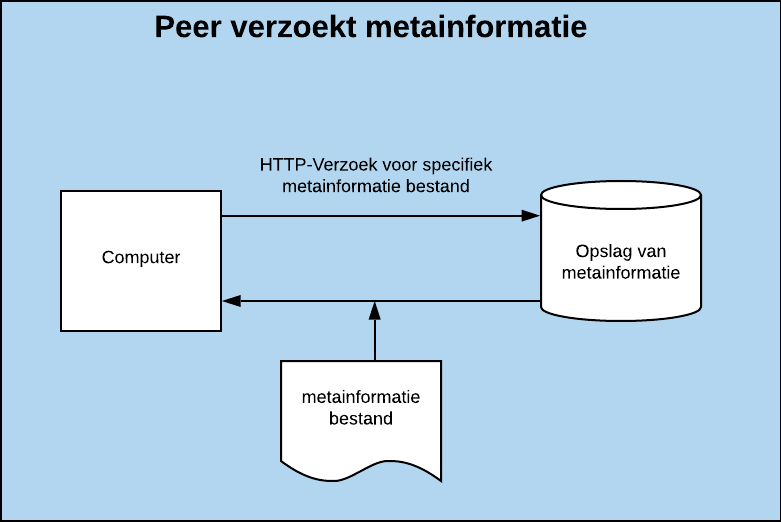
\includegraphics[scale=.4]{torrent-1.png}
\caption[Peer metainformatie stap  - Torrenting 1]{De peer maakt een verzoek aan een opslagplaats voor een metainformatie bestand.}
\end{figure}

Dit metainfo bestand wordt over het algemeen afgehaald van een website of een ftp server. Een gekend voorbeeld van een website die metainfo bestanden ter beschikking stelt is \textit{The pirate bay}\footnote{Het is ook belangrijk om kort te vermelden dat file-sharing controversieel is. Zo is de gekende Torrent indexering website \textit{"The Pirate Bay"} sinds 2011 verboden in België. Dit verbod is er gekomen aangezien file-sharing ook wordt gebruik voor het verspreiden van auteursrechtelijk beschermd materiaal. Niet alleen het Torrent protocol is hiervoor onder vuur komen te staan. Limewire een muziek deel platform gemaakt bovenop Gnutella werd in 2010 verplicht om te sluiten. Het probleem met deze maatregelen is dat ze niet kunnen worden doorgevoerd. Men kan individuele sites namelijk  blokkeren maar doordat de protocollen bovenop P2P netwerken zijn gebouwd is het niet mogelijk ze compleet onbeschikbaar te maken. Er zijn verschillende kopieën van de piratebay nog steeds toegankelijk in België en alternatieve versies van Limewire zijn eveneens beschikbaar. Het is hierbij belangrijk om te onthouden dat de principes en protocollen niet illegaal zijn maar het verspreiden van auteursrechtelijk beschermd materiaal is dat wel.}. Dit bestand bevat essentiële informatie om de rest van het protocol te faciliteren. Het bevat de namen en bestandsstructuur van de verschillende bestanden binnen deze Torrent. Voor elk van deze bestanden is ook een MD5-Hashwaarde voorzien zodat eenmaal het bestand gedownload is de gebruiker kan controleren of het niet beschadigd is geraakt bij het download proces. Er wordt ook een zogenaamde infowaarde en stuklengte voorzien. Deze komen later aanbod. Het belangrijkste element in het metainfo bestand is echter het IP-adres van de \textbf{Tracker}. Deze Tracker is een computer die de andere delen van het protocol gaat overzien en aansturen. Aangezien er één centrale computer nodig is om dit protocol in goede banen te leiden is er dan ook sprake van een hybride netwerk.\\

\begin{figure}[h!]
	\centering
		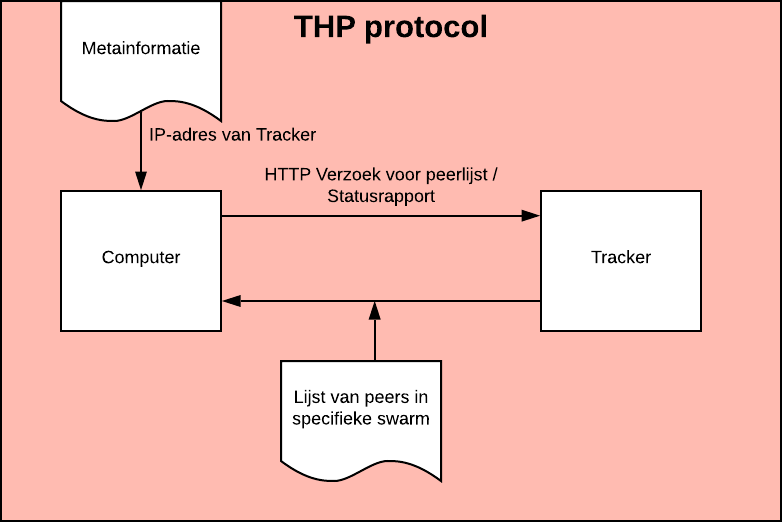
\includegraphics[scale=.4]{torrent-2.png}
			\caption[THP stap - Torrenting 2]{De peer doet een verzoek voor de peerlijst aan de tracker doormiddel van informatie uit het metainformatie bestand.}
\end{figure}
\newpage
Om deze stap te verduidelijken kan er gebruik worden gemaakt van volgend voorbeeld:\\

Bob en Alice maken een Torrent van hun website. Hun website bevat verschillende pagina's en afbeeldingen die zich in een media folder bevinden. Ze stellen een lijst op van deze verschillende bestanden en berekenen voor elk van deze bestanden een MD5-Hash waarde. Bobs computer zal de rest van het protocol coördineren en aldus functioneren als Tracker. Er wordt tot slot een unieke infosleutel voorzien en stuklengte (het is aangeraden deze stuklengte rond 70kb in te stellen). Op basis van deze informatie wordt een metainfo bestand aangemaakt dat wordt beschikbaar gesteld aan de buitenwereld.\\

In de derde stap wilt men toegang verkrijgen tot andere peers die dit bestand bezitten. Men heeft immers andere computers nodig vanwaar men het bestand kan downloaden. De verzameling van computers die een torrent toegankelijk stellen voor het netwerk wordt ook wel een \textbf{swarm} genoemd. Men kan een swarm dan ook zien als een klein netwerk met als functie toegang te verlenen tot een specifieke collectie van bestanden. De functie van de Tracker is om toegang te verschaffen aan deze Swarm en ook informatie hierover bij te houden. Het principe van toegang verschaffen en informatie bijhouden wordt ook wel \textit{THP}(Tracker HTTP protocol) genoemd. De locatie van deze tracker staat vermeld in het metainfo bestand. Om een lijst van peers te krijgen die in een swarm zit, stuurt de computer een HTTP-GET verzoek naar de tracker. In dit verzoek moeten een aantal zaken worden meegestuurd waaronder het IP-adres van de computer, de infosleutel en de poort waarop de communicatie met andere peers kan gebeuren. De Tracker zal vervolgens aan de hand van de infosleutel een lijst van peers terugsturen die de gegeven bestanden ter beschikking stellen.\\

\begin{figure}[h!]
	\centering
		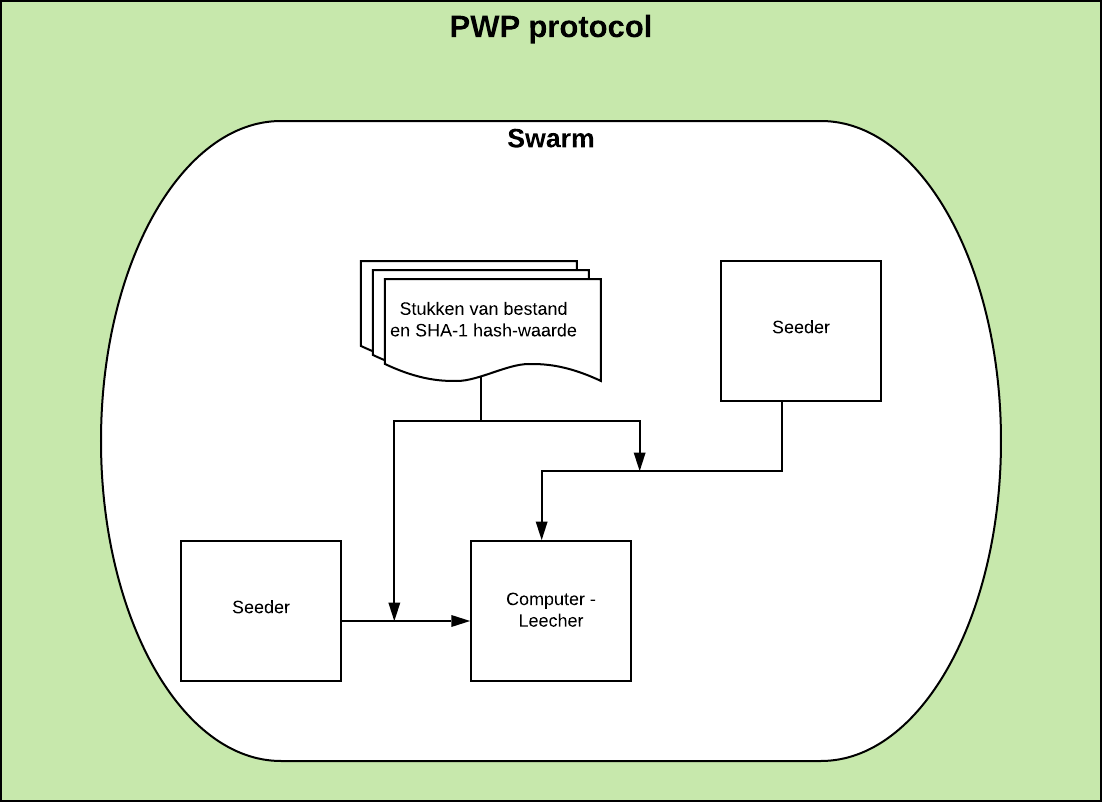
\includegraphics[scale=0.6]{torrent-3.png}
	\caption[PWP stap - Torrenting 3]{De peer verzoekt andere peers voor stukken data en downloadt op die manier de Torrent bestanden.}
\end{figure}
\newpage
Om dit principe te verduidelijken wordt verder gebouwd op bovenstaand voorbeeld:\\

Charlie wil de website van Bob en Alice. Hij heeft van Alice het metainfo bestand ontvangen. Aangezien dit bestand het IP-adres van Bobs computer als Tracker bestempelt wordt er naar deze computer een HTTP-GET verzoek verstuurd. Bob en Alice hebben beiden deze bestanden lokaal staan en vormen aldus samen een swarm. Charlie zal hun IP-adres en poort waarop het verkeer kan verlopen doorgestuurd krijgen en gaat rechtstreeks met beide computers communiceren om de bestanden te downloaden.\\

Er dient opgemerkt te worden dat netwerken en bestanden erg veranderlijk zijn, een computer kan elk moment uitgaan of van het netwerk treden. Het is dus noodzakelijk dat de Tracker een accurate lijst van peers gaat bijhouden in de Swarm. Om dit te bereiken zal een Tracker vragen dat elke peer op een vast tijdsinterval zijn status rapporteert. Zo kan de Tracker accurate informatie voorzien.\\

De computer heeft nu een lijst van verschillende Peers binnen een specifieke swarm. De laatste stap van het protocol is het effectief verkrijgen van de bestanden. De communicatie loopt uitsluitend tussen de verschillende peers zelf. Deze stap wordt ook wel aangeduid als het \textit{PWP} protocol (Peer Wire Message). Bandbreedte en andere beperkingen spelen een grote rol binnen netwerkverkeer. Men wil een peer zo weinig mogelijk belasten. Op die manier stimuleert men de peer om zolang mogelijk op het netwerk te blijven. Het is aldus niet praktisch om volledige bestanden op te vragen van één peer. Stel dat het bestand bijvoorbeeld verschillende gigabytes groot is. Hierdoor zal men het bestand opdelen in verschillende kleine stukken. Deze stukken kunnen individueel worden opgevraagd aan verschillende computers. Op deze manier kan men een bestand van verschillende gigabytes in duizend keer opvragen bij verschillende peers die elk enkele mb doorsturen. De grootte van elk stuk wordt bepaald in het metainfo bestand en staat vastgelegd in de zogenaamde stuklengte. Een ander voordeel van deze fragmentering is dat men individuele stukken kan verifiëren. Elk van deze stukken heeft namelijk zijn eigen SHA-1 hashwaarde. Op die manier kan men gedurende de overdracht van een stuk onmiddellijk nagaan of dit goed is toegekomen en indien er fouten zijn dit klein stuk opnieuw opvragen. Het PWP protocol komt neer op het opvragen en valideren van individuele stukken aan verschillende peers.\footnote{De manier waarop deze stukken worden opgevraagd, ligt buiten de scope van deze bachelorproef. Een goed overzicht wordt gegeven in de tekst van \textcite{Fonseca2005}.} Eenmaal alle stukken zijn gedownload, worden deze samengenomen tot het origineel bestand dat op zijn beurt kan worden gevalideerd aan de hand van MD5.\\

Het Torrent protocol heeft een aantal voordelen. Zoals eerder vermeld is het nog steeds relevant hoewel het van 2002 dateert. Het biedt immers een relatief eenvoudige manier aan om bestanden te downloaden. Door een goede metainformatie indexeringswebsite te gebruiken zoals \textit{The pirate bay} vindt men op eenvoudige wijze de correcte bestanden terug. Dit is bij FTP minder evident.\\

Toch zijn er ook veel technische nadelen verbonden aan het Torrent protocol\footnote{Er zijn ook veel morele implicaties verbonden aan Torrenting maar deze vallen buiten de scope van deze bachelorproef.}:

\begin{itemize}
\item Doordat men gebruik moet maken van een centrale Tracker is er ook één SPOF. Indien de tracker onbereikbaar is dan kan het Torrent protocol niet lang functioneren.\\

\item Het verkrijgen van de metainformatie bestanden is niet evident. Men moet toegang krijgen door middel van een indexeringswebsite of de auteur van de Torrent moet dit bestand doorsturen.\\

\item Volgens \textcite{Thanekar2010} kunnen bestanden permanent verloren gaan. Dit is het geval indien er geen Seeders of volledige kopieën beschikbaar zijn.\\

\item Peers communiceren rechtstreeks met elkaar over TCP. Hiervoor heeft men elkaars IP-adres nodig. Dit leidt er dus toe dat men niet anoniem is bij de download en upload van bestanden.\\

\item Er is weinig stimulans voor een peer die bestanden downloadt om deze ook toegankelijk te stellen voor het netwerk en de rol van Seeder op zich te nemen. Om dit probleem te vermijden wordt een zogenaamde \textit{Tit for tat} beleid gehanteerd. Hierbij kunnen peers enkel bestanden downloaden indien ze effectief ook bijdragen aan de download van anderen.\\

\item Tot slot moet men ook rekening houden dat er geen manier is om volledig te verifiëren wat men downloadt. Men kan nagaan of het bestand hetzelfde is als dat in de metafile. Dit is echter geen garantie dat het bestand veilig is en de relevante informatie bevat. 
\end{itemize}

Vele van deze problemen stellen zich ook in het klassieke Client-Server model.

\subsubsection{Gnutella}
\label{Gnutella}
Zoals uitgelegd in \ref{torrenting} is het Bit-Torrent protocol niet volstrekt gedecentraliseerd. Er is immers een centrale component (de Tracker) noodzakelijk om de verbinding tot het netwerk van peers tot stand te brengen. Indien deze centrale component onbereikbaar is kan er geen verbinding tot stand worden gebracht. Om dit probleem te omzeilen moet er een manier zijn om in een volstrekt gedecentraliseerde manier bestanden te delen met elkaar. Hiervoor kan men gebruik maken van Gnutella.\\

Gnutella is een protocol met als doelstelling het verspreiden en toegankelijk stellen van bestanden in een volledig gedecentraliseerd netwerk. Het protocol bereikt dit door het versturen van verschillende types van berichten over een TCP/IP connectie. De uitleg over dit protocol is gebaseerd op de \textit{draft RFC} die wordt onderhouden door \textcite{Klingberg2002}. Om het protocol te kunnen gebruiken zijn er aantal stappen die een peer moet overlopen:

\begin{itemize}
\item De peer ($p_1$) zoekt toegang tot het netwerk doormidden van een connectie aan te gaan met een peer die reeds met netwerk verbonden is. Voor de duidelijkheid wordt deze initiële peer bestempeld met het symbool $p_0$ doorheen deze tekst.\\
\item De peer ($p_1$) verkrijgt meer informatie over het netwerk door berichten te versturen aan deze peer ($p_0$).\\
\item De peer $p_1$ gaat connecties aan met andere peers. Vervolgens kan $p_1$ bestanden gaan delen of opvragen aan het netwerk.\\
\item De peer $p_1$ is nu een volwaardig lid van het netwerk en kan andere peers toegang verschaffen. $p_1$ kan aldus de rol van initiële peer $p_0$ op zich nemen.
\end{itemize}


\textbf{Verbinden op het netwerk}\\

Zoals eerder aangehaald moet een peer zich verbinden op het Gnutella netwerk om bestanden te kunnen opvragen. Een peer kan toetreden door contact te leggen met een peer die reeds verbonden is op het netwerk. Wil bijvoorbeeld Bob bestanden delen op het netwerk zal hij Alice moeten contacteren die al reeds verbonden is. Voor leesgemak wordt doorheen deze tekst het begrip \textbf{verzoeker} gebruikt als er wordt verwezen naar de peer die toegang wilt tot het netwerk. De peer die toegang verschaft wordt bestempeld als \textbf{aanbieder}.\\


\subsection{IPFS}
\label{IPFS}
\subsubsection{Inleiding}
IPFS is een modern file-sharing protocol dat veel van de tekortkomingen van Bit-Torrent en Gnutella oplost -zie \ref{vergelijking-FS}. Het is ook het protocol dat gaat worden gebruikt in het opstellen van de POC. De uitleg in dit hoofdstuk is afkomstig van de officiële documentatie \autocite{}, Github Repository \autocite{} en video's(\autocite{} , \autocite{}).\\

Allereerst wordt het concept van een \textbf{CID} en \textbf{Content based addressing} toegelicht. Dit concept wordt namelijk gebruikt om bestanden te gaan identificeren binnen de POC. 

\subsubsection{Content Based Adressing}
%Hellemaal opnieuw te beginnen, Hoe worden bestande opgeslaan op IPFS.
\label{CBA}
\textbf{Wordt nog verder aangevuld}
 De opzet van het protocol beperkt zich niet louter tot bestandsoverdracht. Ze beschrijven zichzelf als een gedistribueerd bestandssysteem dat een alternatief biedt voor de manier waarop er op het internet informatie wordt opgevraagd. Wat wordt daar echter mee bedoeld?\\

IPFS heeft als doelstelling om alle bestanden op het netwerk te gaan verspreiden over verschillende peers. Deze bestanden kunnen vervolgens eenvoudig worden opgevraagd en weergegeven in een webbrowser. Een peer kan vervolgens rechtstreeks aan het netwerk deze bestanden gaan opvragen. In tegenstelling tot Bit-Torrent is er aldus geen sprake van Trackers of Swarms. Gnutella heeft echter dezelfde benadering. Dus wat maakt IPFS uniek?\\

Volgens IPFS is er een probleem met de manier waarop er klassiek wordt gezocht naar bestanden. Stel bijvoorbeeld onderstaand scenario:\\

Bob wilt graag een nieuwe achtergrond en gaat opzoek naar een afbeelding van een Capybara. Hij vindt twee afbeelding op google van een mooie Capybara en slaat vervolgens de links op. Drie dagen erna bezoekt hij nog eens de links, één van deze links lijdt naar een 404 pagina. De afbeelding is immers verwijderd. De andere link lijdt tot zijn verbazing tot een afbeelding van een Tapir.\\

Dit is eveneens een voorbeeld van \textbf{Location based addressing}. Location based addressing(=lba) is het principe dat men een bestand gaat opvragen aan de hand van waar dit bestand bevind. Zo gaat de link abc.com/cat.jpg het bestand cat.jpg gaan opvragen aan de server van abc.com. Bovenstaand voorbeeld illustreert ook onmiddellijk drie problemen met lba:

\begin{enumerate}
\item Informatie kan gemakkelijk offline worden gehaald. Er is geen enkele garantie dat afbeeldingen, websites en andere bestanden beschikbaar blijven.\\
\item Er wordt veel vertrouwen gesteld in servers dat de informatie die men opvraagt correct is. Omdat een bestand een bepaalde naam heeft wilt dat niet noodzakelijk iets zeggen over de inhoud ervan.\\
\item Informatie kan eenvoudig worden gewijzigd. De afbeelding die gisteren nog een capybara was kan veranderd zijn in een afbeelding van een Kat.\\
\end{enumerate}

Het zijn deze problemen die worden aangepakt met Content Based Adressing (=CBA),IPFS en het concept van een CID. Binnen CBA worden bestanden opgevraagd aan de hand van hun inhoud. Bij een klassieke url moet immers zowel de naam van de server (of het ip-address) alsook de naam van het bestand in kwestie gekend zijn. CBA vervangt dan ook het concept van een URL door een uniek identificatie nummer dat gebaseerd is op de inhoud van het bestand. Dit uniek identificatie nummer wordt een CID genoemd. Het is belangrijk dat de verschillende elementen van een CID worden besproken. Op die manier kan er worden geïllustreerd wat de verschillende eigenschappen zijn van CBA en hoe deze kunnen worden toegepast binnen IPFS.\\

Om het principe van een CID te kunnen uitleggen kan er worden gekeken wat er exact gebeurd op het moment dat er een bestand op het IPFS netwerk wordt gezet. Op het moment dat een bestand wordt geplaatst op het IPFS netwerk zal het eerst lokaal worden opgedeeld in stukken van maximaal 256kb groot. Voor elk van deze delen alsook het hoofdbestand wordt een hashwaarde berekend -voor meer informatie zie \ref{hashing}-. IPFS gebruikt SHA2-256. De waarde die verkregen wordt uit deze functie wordt ook wel de \textbf{digest} genoemd.\\

\begin{figure}[h!]
	\centering
		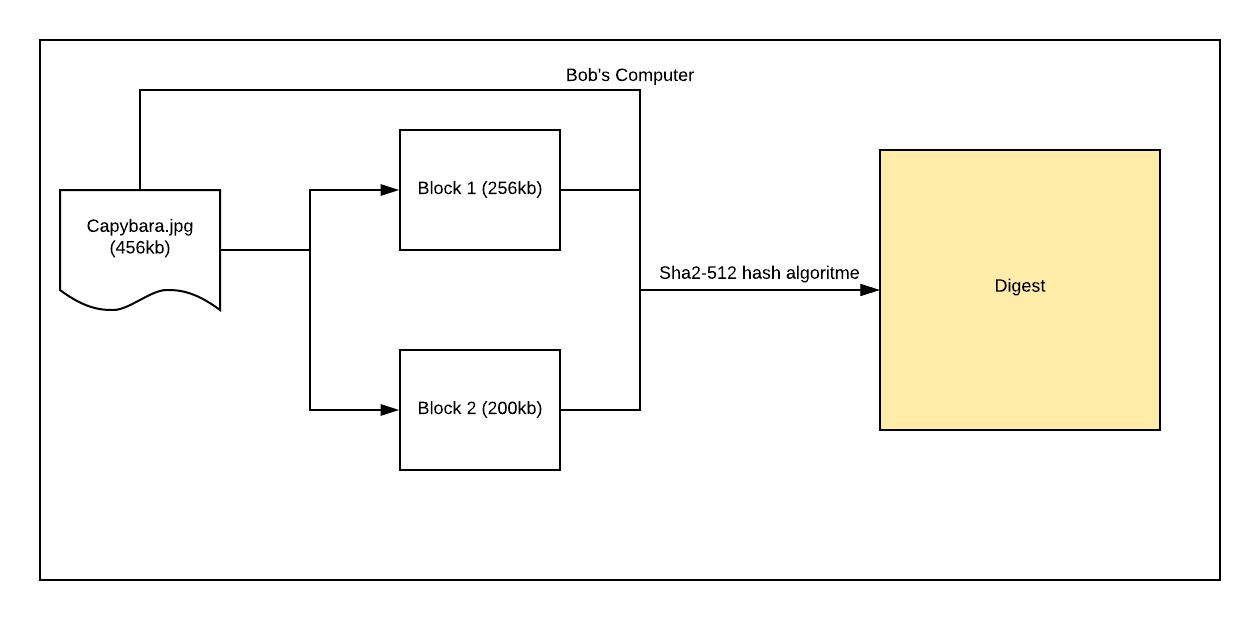
\includegraphics[scale=0.6]{ipfs-1.png}
	\caption[IPFS - Stap 1]{Bestand wordt opgedeeld in verschillende blokken. Elk van deze blokken en het bestand zelf worden vervolgens door SHA2-512 gehashed en men verkrijgt aldus een digest. }
\end{figure}

Op basis van de hash van de individuele blokken wordt vervolgens een CID opgesteld.  

%\subsubsection{Het probleem van altruïsme}
%Een groot probleem binnen file-sharing protocollen is het probleem van de Ratio. Binnen file-sharing Torrent protocollen kent men het onderscheid tussen een \textbf{Leecher} en een \textbf{Seeder}. Een peer die een bestand download wordt ook wel een Leecher genoemd en een node die een bestand beschikbaar stelt voor deze Leechers noemen we een Seeder. De ratio is bijgevolg het aantal seeders ten opzichte van het aantal leechers. Bij veel niet gesuperviseerde netwerken is dit ratio eerder laag -sommige netwerken legen namelijk verplichtingen op aan deelnemers zodat bestanden vlot toegankelijk blijven-. Veel leechers kiezen er namelijk voor om enkel bestanden te downloaden. Indien er geen Seeders meer zijn voor een bestand is dit in essentie ontoegankelijk geworden. Deze problemen kunnen worden vermeden door een voldoende groot netwerk te kiezen. Dit probleem doet zich echter ook voor bij protocollen zoals Gnutella en IPFS. Er is namelijk geen verplichting om bestanden beschikbaar te stellen. Eenmaal de peer de gewenste bestanden heeft binnen gehaald is er geen stimulans meer deze te delen. Het is dan ook aangewezen om een groot aantal deelnemers te hebben. Hoe meer Peers binnen een netwerk hoe meer toegankelijk het wordt en hoe meer kans dat deze peers ook effectief bestanden zullen beschikbaar stellen. Vandaar dat het aangewezen is om een reeds bestaand netwerk te gebruiken ten opzichte van een eigen implementatie.\\
\section{vergelijking van de verschillende file-sharing protocollen}
\label{vergelijking-FS}
\textbf{Moet nog aangevuld}

\section{Blockchain principes}
\subsection{Inleiding}
Blockchain is een gedecentraliseerde opslagoplossing. Blockchain werd in 2009 ontworpen door \textcite{Satoshi2009} en vormt de basis van Bitcoin. Zoals vermeld in het Witboek van \textcite{Satoshi2009} is de doelstelling van Bitcoin om een elektronisch peer-to-peer betalingssysteem te voorzien. Het idee van Nakamoto was vooral revolutionair aangezien het een manier biedt om binnen een P2P netwerk gegevens op te slaan en deze gegevens ook te valideren. Het probleem dat Bitcoin oplost voor P2P netwerken staat ook wel bekenD als het \textit{Byzantine Generals’ Problem}.\\

Dit probleem kan als volgt worden beschreven: Drie generalen moeten beslissen om een stad aan te vallen. Ze kunnen enkel communiceren via koeriers die tussen de verschillende generalen berichten overbrengen. De drie generalen moeten het eens geraken om de stad aan te vallen of met rust te laten. Eenmaal de aanval is ingezet is er geen manier om terug te trekken \autocite{Peter2018}. Aanvankelijk lijkt dit probleem triviaal. Ze sturen alle drie een bericht naar elkaar en bereiken een consensus door twee derde meerderheid. Toch is dit probleem complexer: wat als de boodschapper niet te vertrouwen is bijvoorbeeld? Wat als er een generaal is die twee verschillende stemmen uitbrengt?\\

Dit probleem demonstreert dat het niet eenvoudig is om tot een consensus te komen in een systeem waar ieder als gelijke wordt gezien. Er is immers één rotte appel nodig om de hele consensus te beïnvloeden. Blockchain is innoverend omdat het een consensus algoritme biedt om binnen een P2P netwerk -waar iedere node als gelijke wordt gezien- boodschappen en gegevens op te slaan. Deze boodschappen en gegevens worden ook wel \textbf{transacties} genoemd.\\

Hoe kadert blockchain binnen de POC die in deze bachelorproef wordt ontwikkeld? Zoals eerder vermeld -zie \ref{Duiding_IPFS}- bestaat een versiebeheersysteem niet enkel uit bestanden maar ook uit een logboek. Dit logboek is in essentie een overzicht van alle wijzigingen in de bestanden. Dit logboek moet worden opgeslagen en kunnen worden aangepast op een P2P netwerk. Hiervoor kan er worden gebruik gemaakt van een blockchain.\\

\subsection{Basis principes van een blockchain}
In deze sectie wordt blockchain uitgelegd aan de hand van het originele voorstel door \textcite{Satoshi2009} en de video gepubliceerd door \textcite{Blue2017}.\\

In het kort gesteld is blockchain een geheel van met elkaar verbonden blokken van transacties. Dit systeem van onderling verbonden blokken wordt ook wel een \textbf{ledger} genoemd. Elke peer heeft ten allen tijden een kopie van deze ledger. Een transactie is een bepaalde set van data. In het geval van bitcoin is dit een overschrijving. Een voorbeeld van een transactie op het bitcoin netwerk is Alice geeft Bob 25 bitcoins. Een blok is aldus een lijst van transacties. Om dit principe te verduidelijken, kan er gebruik worden gemaakt van onderstaande grafische voorstelling:\\

\begin{figure}[h!]
	\centering
		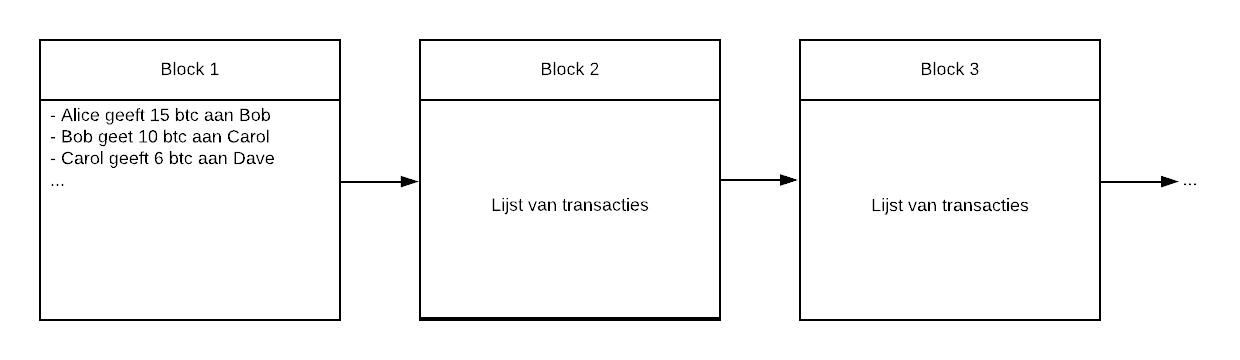
\includegraphics[scale=0.4]{blockchain-1.png}
	\caption[Blockchain - Voorstelling 1]{De blockchain bestaat uit onderling verbonden blokken. Een blok bevat een lijst van transacties.}
	\label{blocks}
\end{figure}

Hoe worden deze transacties gevalideerd? Hoe weten we bijvoorbeeld dat Alice wel degelijk 15 bitcoins aan Bob geeft? Dit gebeurt door \textbf{asymmetrische cryptografie}. \textcite{Farah2012} stellen dat asymmetrische cryptografie gebruik maakt van twee sleutels: enerzijds de sleutel die gebruikt wordt bij het encrypteren van een bericht, anderzijds de sleutel die gebruikt wordt bij het decrypteren. Als zowel de encryptiesleutel en het hashingalgoritme gekend zijn dan is het computermatig onwaarschijnlijk dat de decryptiesleutel kan worden achterhaald. De encryptiesleutel wordt ook wel de \textbf{publieke sleutel} genoemd. De decryptiesleutel wordt de \textbf{privé sleutel} genoemd. De privé sleutel is enkel in handen van één persoon en mag niet gedeeld worden met andere. De publieke sleutel is toegankelijk voor iedereen. Hoe wordt dit principe gebruikt om te verifiëren dat Alice wel degelijk de verzender is van het bericht?\\

Alice kan bewijzen dat ze een transactie heeft goedgekeurd door deze transactie te ondertekenen met haar privé sleutel. Dit principe is gelijkaardig aan de manier waarop officiële documenten worden ondertekend. Bij handtekeningen op officiële documenten kan er worden geverifieerd dat deze ondertekend zijn door een bepaald persoon door middel van zijn/haar handschrift. Bij digitale handtekeningen kunnen we verifiëren dat ze zijn ondertekend door een bepaald privé sleutel van een persoon. Dit gebeurt door de corresponderende publieke sleutel, de handtekening en het originele bericht.\footnote{Deze uitleg is nogal kort door de bocht. Asymmetrische encryptie is een uitgebreid concept. Voor meer informatie hoe deze wordt toegepast binnen bitcoin zie: $https://learnmeabitcoin.com/beginners/digital_signatures$} Dit wordt geïllustreerd in de onderstaande grafiek:

\begin{figure}[h!]
	\centering
		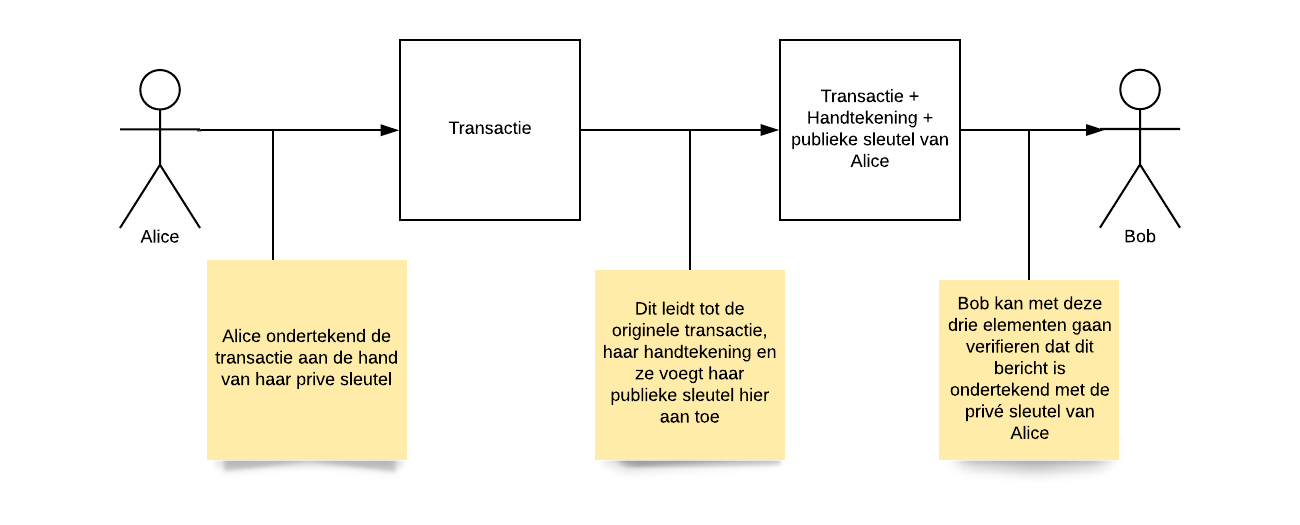
\includegraphics[scale=0.4]{blockchain-2.png}
	\caption[Blockchain - Voorstelling 2]{Alice ondertekent transacties aan de hand van haar privé sleutel.}
\end{figure}

Elke peer heeft zoals reeds eerder vermeld zijn eigen kopie van de ledger. Dit wilt zeggen dat elke deelnemer van het netwerk ten allen tijden een volledige lijst van transacties heeft. Een voordeel van een volledige lijst van transacties bij te houden is dat er kan geverifieerd worden dat Alice wel degelijk over 15 bitcoin beschikt. Alice kan aldus niet meet uitgeven dan ze reeds heeft. Op het moment dat Alice of Bob een transactie uitvoeren, zal deze dus over heel het netwerk worden verspreid.  Al deze transacties worden gebundeld onder de vorm van blokken -zie grafiek \ref{blocks} -. Door bijvoorbeeld twee keer dezelfde blokken toe te voegen of bepaalde blokken eruit te halen kan een individuele gebruiker blockchain en transacties manipuleren.  Om dit te vermijden wordt het concept van een consensus algoritme gebruikt. Om meer specifiek te zijn wordt binnen bitcoin het zogenaamde \textbf{Proof of Work} algoritme gebruikt.\\

Proof of work is een concept dat is ontwikkeld door \textcite{Dwork}. Proof of work vereist het oplossen van een uniek wiskundig probleem alvorens een bepaalde handeling mag worden uitgevoerd. In het artikel van \textcite{Dwork} werd dit principe gebruikt om spam te vermijden. Indien een computer voor elke e-mail een wiskundig probleem moest oplossen is het praktisch onmogelijk om duizenden en duizenden e-mails te versturen. Hoe kadert dit principe binnen blockchain?\\

Bitcoin gebruikt het proof of work (=PoW) principe voor het valideren van blokken. Pas als het volgende wiskundig probleem is opgelost, mag een blok worden toegevoegd aan de blockchain. Binnen cryptografie speelt het concept van hashing een grote rol - zie \ref{hashing} -. Een eigenschap van deze hashes is dat het wiskundig onwaarschijnlijk is om gegeven een bepaalde hashwaarde de originele input waarde te vinden. Het is echter relatief eenvoudig om een bepaalde input waarde te hashen. Het PoW algoritme gebruikt deze eigenschappen door volgend wiskundig probleem op te stellen:\\

Bereken de hashwaarde gebruik makend van alle transacties + een bepaald getal. De resulterende hash moet x-aantal nullen bevatten in het begin van de hashcode. Het probleem bestaat er aldus uit om het getal te vinden dat ervoor zorgt dat de resulterende hash met x-aantal nullen begint.  Om dit principe nog eens te verduidelijken stel onderstaand scenario:\\

Alice ontvangt 200 transacties. Ze bundelt deze samen tot een blok. De wiskundige opgave bestaat er aldus uit om een getal x te vinden (ook wel de \textbf{nonce} genoemd) dat samen met de lijst van transacties door het SHA-256 een hash code oplevert met n-aantal nullen in het begin.\\

De volgende grafiek verduidelijkt dit scenario:

\begin{figure}[h!]
	\centering
		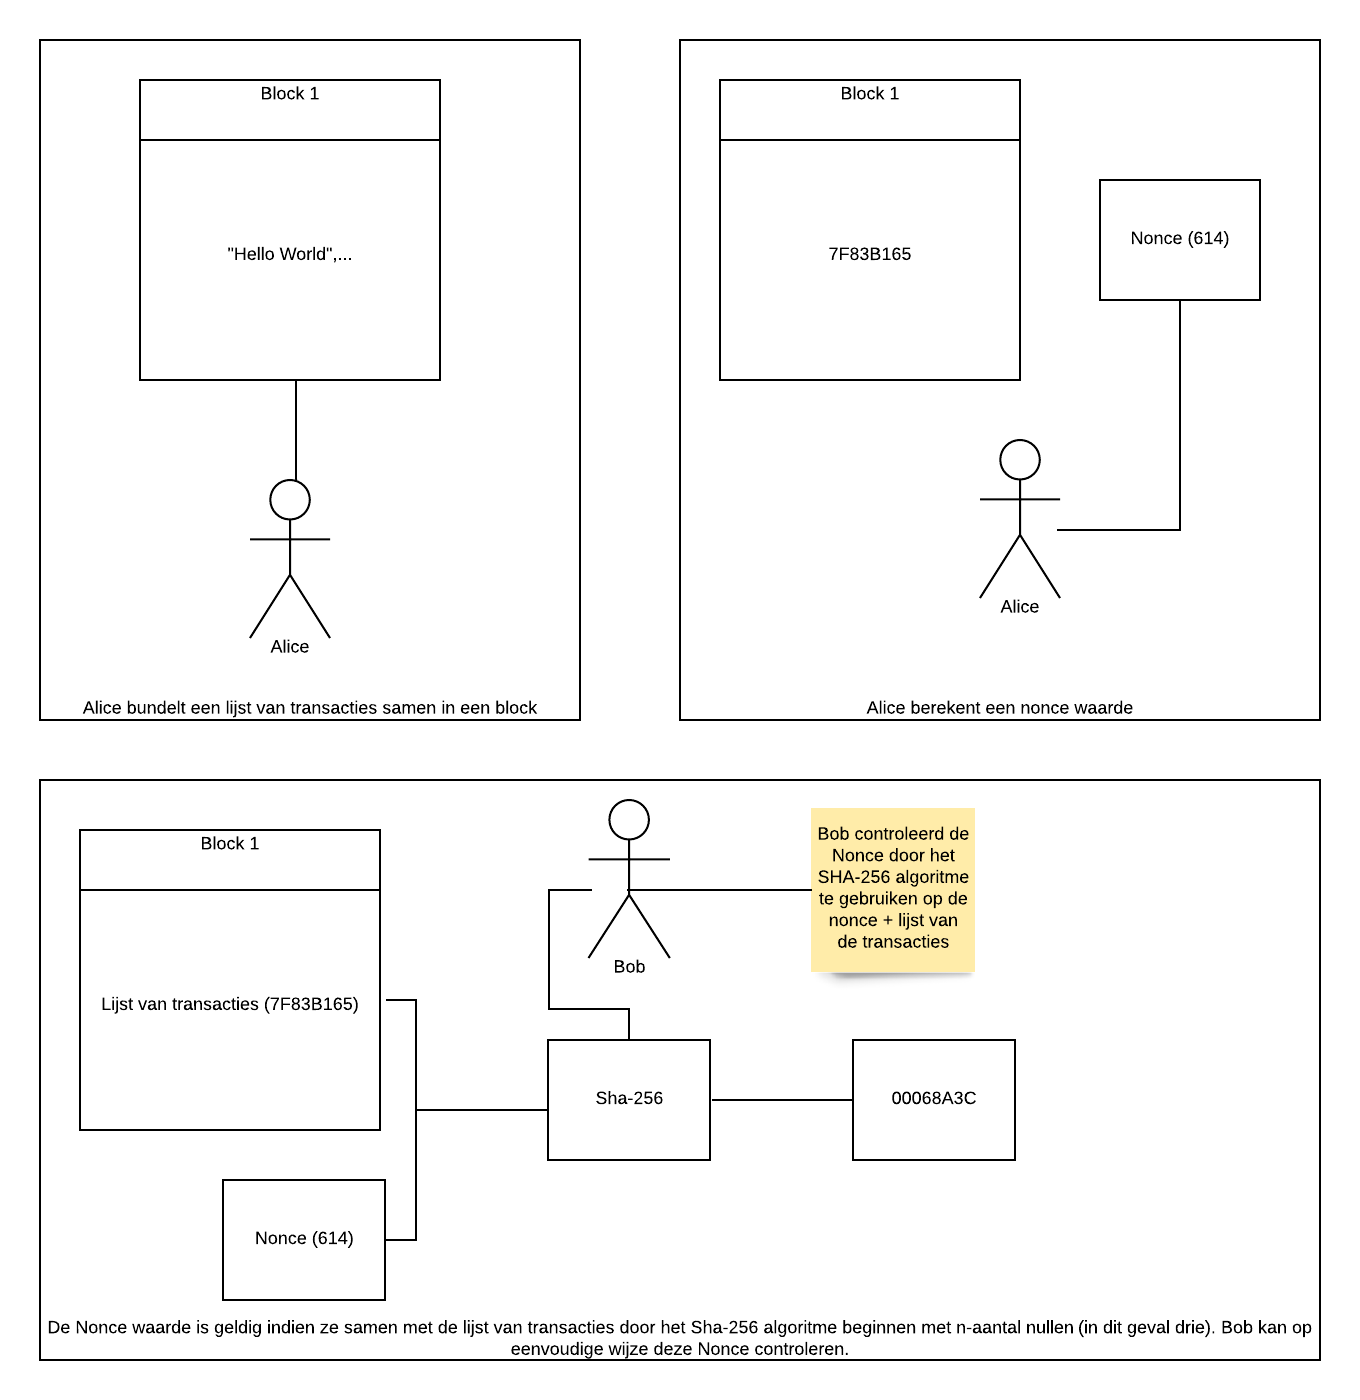
\includegraphics[scale=0.3]{blockchain-3.png}
	\caption[Blockchain - Voorstelling 3]{Voorstelling van een hash-puzzel.}
\end{figure}

\newpage

Het proof of work algoritme heeft twee verschillende eigenschappen:

\begin{enumerate}
	\item De nonce kan enkel worden gevonden door alle verschillende mogelijkheden te berekenen Zoals vermeld in \ref{hashing} kan men niet via de gewenste uitkomst de inputwaarde berekenen. Men kan dus niet simpelweg een getal met het aantal vereiste 0-bits omzetten naar een corresponderende inputwaarde.
	\item De moeilijkheidsgraad voor het algoritme is rechtstreeks verbonden met het aantal nullen dat vereist is in het begin van de resulterende hashwaarde. Dit is immers ook logisch. Stel bijvoorbeeld dat de resulterende hashwaarde 10 bit lang is en slechts één 0-bit vereist vooraan dan zijn er $2^9 = 512$ toegestane waarden. Wordt deze vereiste op vijf 0-bits gelegd dan zijn er slechts $2^5 = 32$ mogelijke uitkomsten.
\end{enumerate}

Er kan dus gesteld worden dat indien een peer een bepaalde nonce waarden heeft berekend deze een significant rekenkundige taak heeft verricht. Hoe zorgt het Proof Of Work algoritme nu echter voor data integriteit binnen een blockchain netwerk. Anders gesteld hoe zorgt dit algoritme ervoor dat fraude onwaarschijnlijk is.\\

De echte kracht van blockchain ligt in het feit dat de blokken onderling zijn verbonden. Concreet wilt dit zeggen dat de oplossing uit het PoW algoritme wordt opgenomen in het volgende blok. Volgende grafiek illustreert dit principe:

\begin{figure}[h!]
	\centering
		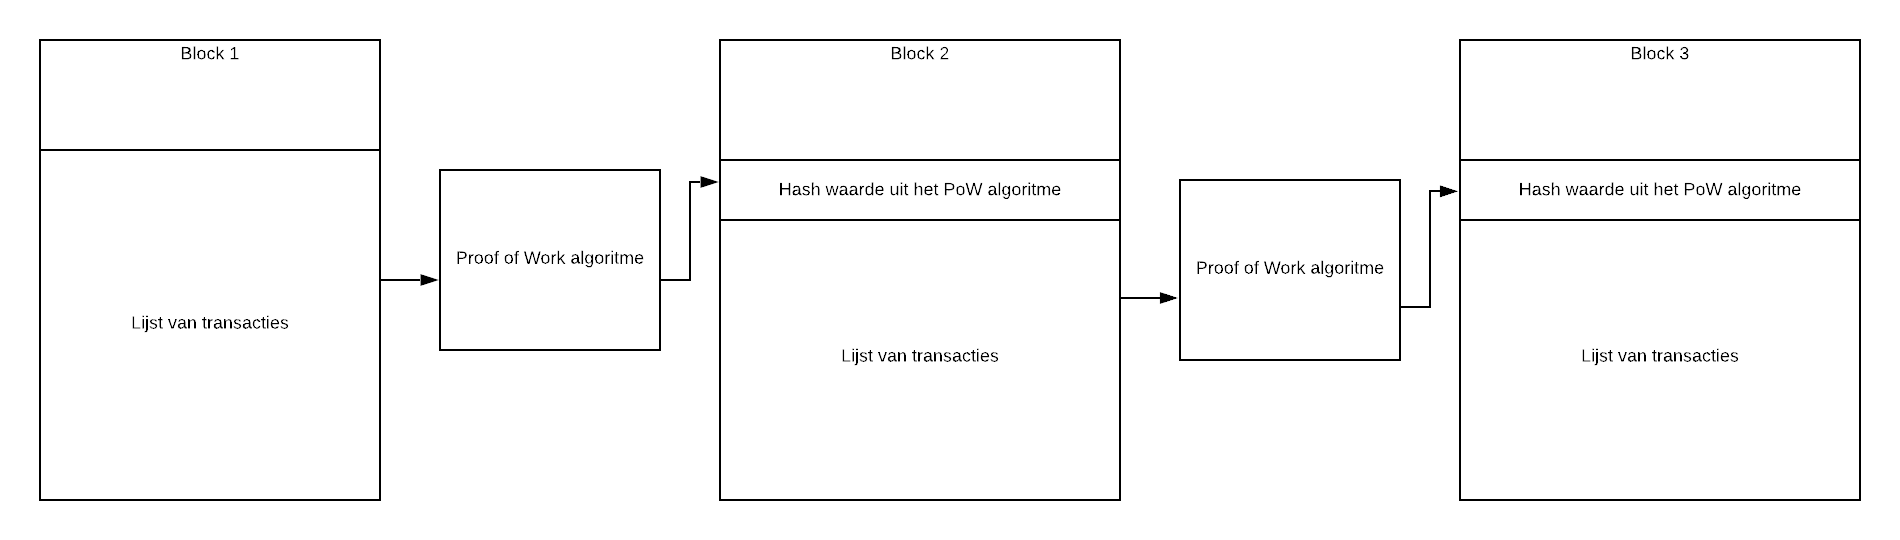
\includegraphics[scale=0.2]{blockchain-4.png}
	\caption[Blockchain - Voorstelling 4]{De blockchain is een verzameling van blokken die onderling verbonden zijn.}
\end{figure}

Dit maakt het vervalsen van transacties uitermate moeilijk om de volgende reden:\\

Stel dat er momenteel 85 blokken aanwezig zijn op de Blockchain. Bob wil blok 42 veranderen. Hiervoor berekent hij opnieuw de nonce waarde. Bob stuurt dit nieuwe blok naar alle andere peers. Deze peers zitten momenteel op blok nummer 85 en zullen het nieuw blok aldus niet opnemen. \textbf{De langste keten is immers correct}. Het blok dat Bob heeft gestuurd, bevat de PoW hash van block 41 en dus niet de meest recente PoW hash waarde. Bob zal dus de overige 44 blokken ook moeten berekenen. Tegen de tijd dat Bob al deze blokken heeft berekend, is het netwerk hoogstwaarschijnlijk al veel verder. Tenzij Bob sneller dan alle andere peers deze nonce waarde kan berekenen is het vervalsen haast onmogelijk.\\

Alle bovenstaande principes vormen de achterliggende technologie van blockchain netwerken. Een korte definitie luidt dus als volgt: blockchain is een manier om in een gedecentraliseerd systeem aan dataopslag te doen. Het is een aaneenschakeling van lijsten van transacties. Hierbij wordt een Proof of Work algoritme gebruikt om ervoor te zorgen dat frauduleuze transacties onwaarschijnlijk zijn.

\subsection{Blockchain mining}
Om deel te nemen aan een blockchain netwerk moet men ten alle tijden een recente kopie hebben van de ledger. Vervolgens kan men transacties maken en deze gaan valideren. Het is hierbij belangrijk om te onthouden dat \textbf{transacties valideren geen vereiste} is om transacties aan te maken. Peers die actief transacties valideren aan de hand van het Proof-of-work algoritme worden \textbf{miners} genoemd. Peers die deelnemen aan het netwerk worden doorheen deze tekst aangeduid als \textbf{participanten}. Het is de taak van miners om transacties door andere peers te bundelen in blokken en vervolgens het PoW algoritme toe te passen. Eenmaal een blok is gevonden, wordt deze verspreid over het netwerk (over zowel participanten als andere miners). De volgende grafiek verduidelijkt het verschil tussen een participant en een miner:

\begin{figure}[h!]
	\centering
		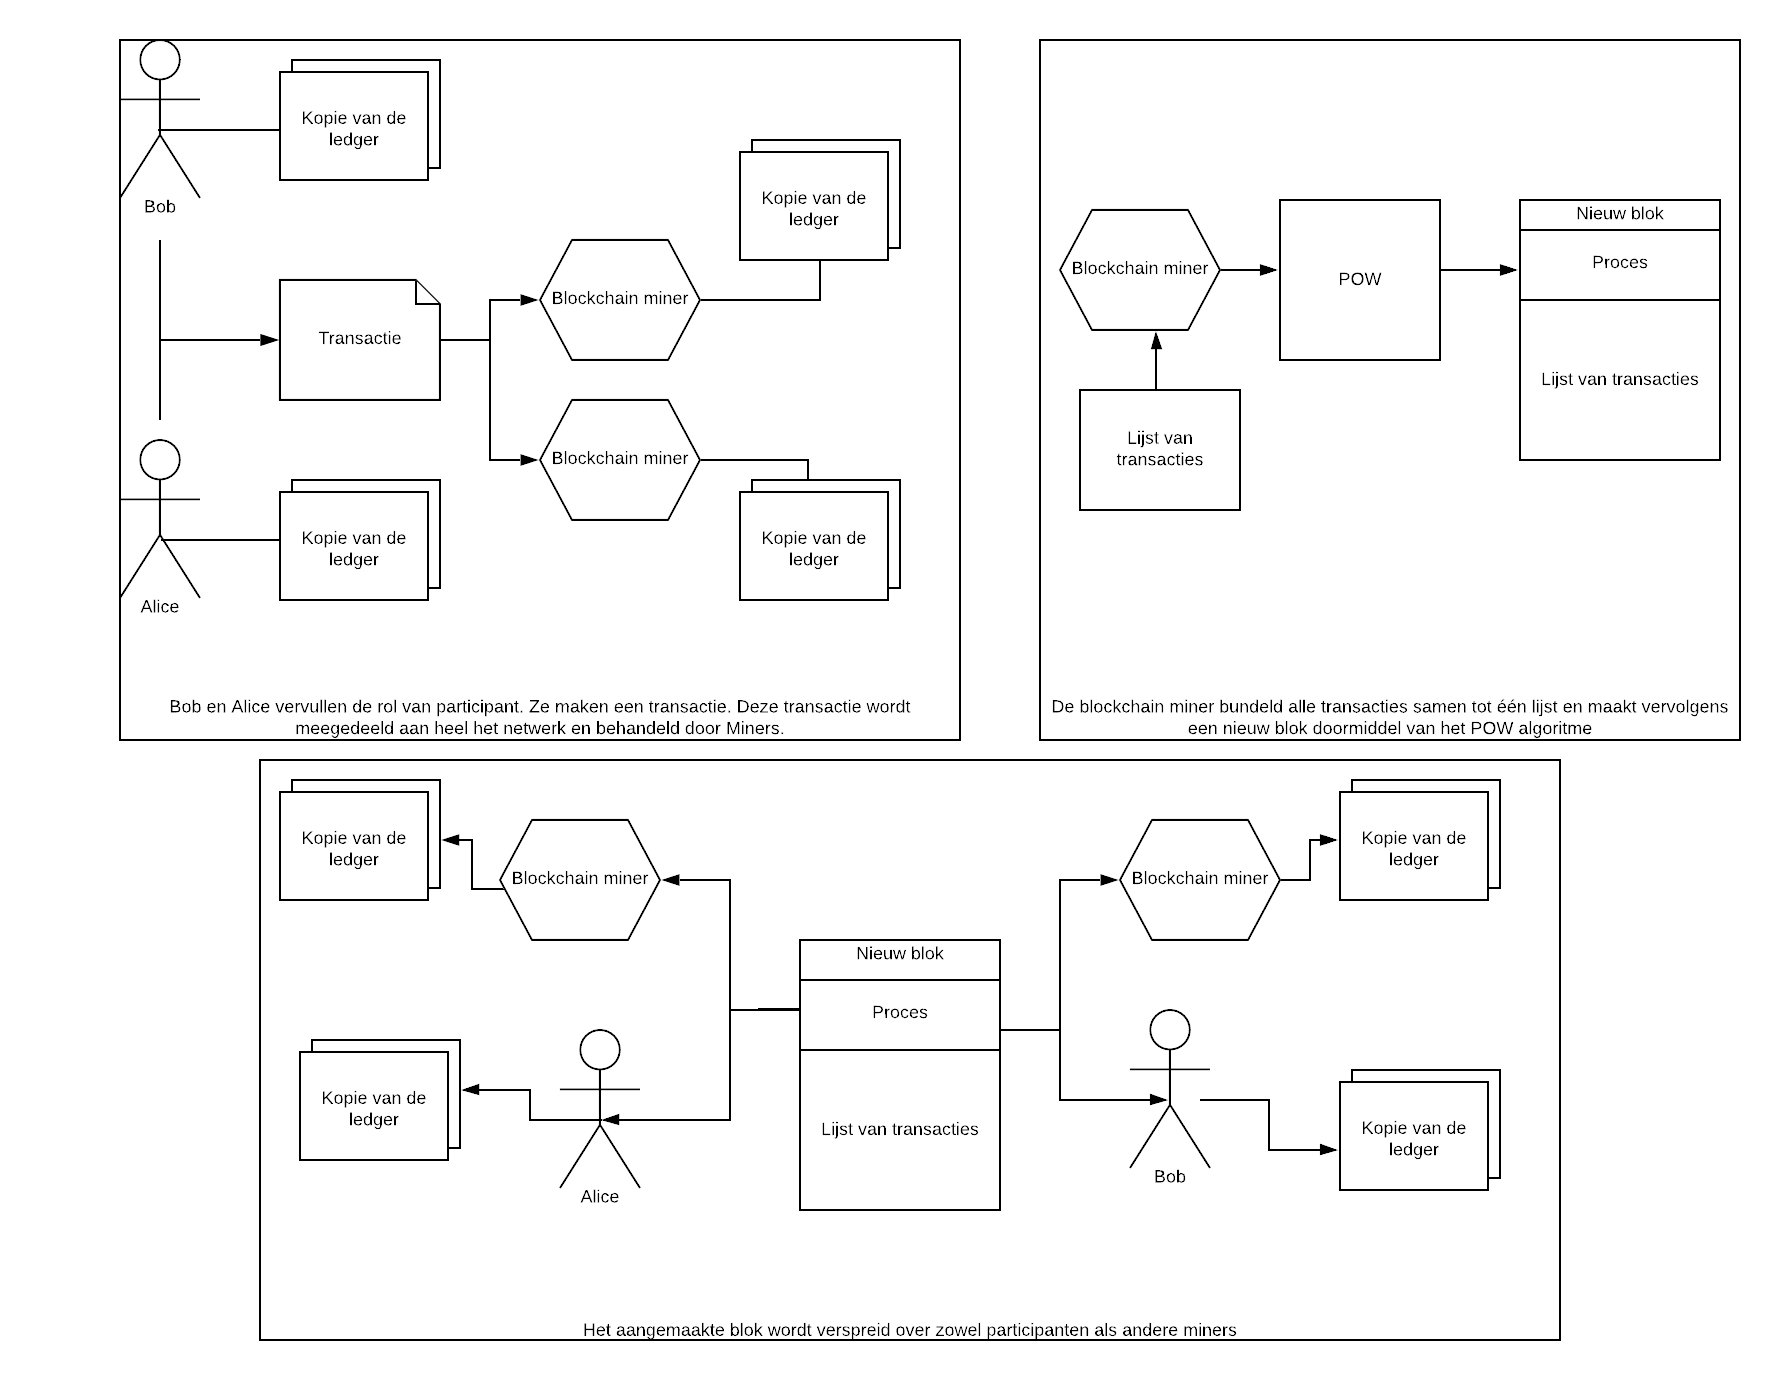
\includegraphics[scale=0.2]{blockchain-5.png}
	\caption[Blockchain - Voorstelling 5]{Een demonstratie van het verschil tussen miners en participanten.}
\end{figure}
\newpage

Zoals hierboven vermeld is het verifiëren van blokken niet verplicht om deel te nemen aan het netwerk. Waarom zouden miners hun tijd en energie in dit proces steken? Ze worden beloond voor het verifiëren aan de hand van een \textbf{block reward}. Wanneer ze een transactielijst samenstellen voegt het bitcoin protocol een speciale transactie eraan toe. Deze transactie wijst een aantal bitcoin toe aan de miner van dit blok. Slaagt de miner er aldus in om dit blok te verifiëren krijgt hij het aantal bitcoin van deze transactie.\\

Zoals hierboven vermeld worden er dus nieuwe munten in circulatie gebracht door het PoW algoritme. Dit is zeker belangrijk als men realiseert dat er geen centrale autoriteit is die deze munt in circulatie brengt. In België bijvoorbeeld wordt de hoeveelheid geld in circulatie beheerd door de Nationale Bank. Hierdoor is er echter een probleem. Mocht het verificatie proces te snel gaan worden er teveel munten in omloop gebracht wat leidt tot het principe van inflatie. Hoe verloopt dit bij Bitcoin?\\

Er zijn drie manieren waarop bitcoin en andere varianten hun geldstroom beheren:

\begin{enumerate}

\item Zoals eerder vermeld is de moeilijkheidsgraad en tijd die het duurt voor het verifiëren rechtstreeks afhankelijk van het aantal 0-bits vereist in het PoW algoritme. Het bitcoin algoritme past dit aantal 0-bits automatisch aan zodat er gemiddeld één blok wordt aangemaakt elke tien minuten. Er worden aldus niet teveel nieuwe munten in omloop gebracht.\\

\item De grootte van een blok is beperkt tot 1 megabyte. De reden hier achter is dat iedere peer een kopie moet bijhouden van de ledger. Opslagruimte is namelijk beperkt. Daarom kan een blok enkel om en bij de 2400 transacties bevatten. Als men weet dat er één blok elke 10 minuten wordt aangemaakt is het aantal transacties aldus min of meer constant. Het bitcoin netwerk is in staat om ongeveer 14.400 transacties te verwerken per uur.\\

\item Het aantal munten dat een miner krijgt voor het verifiëren van een transactie wordt ook wel de \textbf{block reward} genoemd. Deze block reward wordt automatisch gehalveerd elke 210.000 blokken (ongeveer 4 jaar). Hierdoor wordt het aantal nieuwe munten in circulatie verminderd.\\
\end{enumerate}

Zoals hierboven vermeld is het aantal transactie gelimiteerd tot ongeveer 14.400 transactie per uur. Hierdoor is het dus niet duidelijk dat wanneer een participant een transactie verstuurt deze ook effectief snel zal verwerkt worden. Om miners aan te sporen hun transacties te versnellen kunnen participanten ook een \textbf{transactiekost} aan hun transactie toevoegen.  Dit is een kleine optionele kost die participanten toevoegen en die rechtstreeks naar de miner gaat indien deze transactie verwerkt wordt.

\subsection{Ethereum}
Volgens \cite{EthFound2020} is Ethereum een open-source platform voor het schrijven van gedecentraliseerde applicaties. Op dit platform wordt gebruik gemaakt van blockchains. Het idee komt van Vitalik Buterin en werd geformaliseerd in een Witboek gepubliceerd in 2013. De volgende uitleg is dan ook gebaseerd op dit Witboek \cite{Buterin2015}.\\

Het bitcoin protocol is gebouwd bovenop blockchain technologie. Het biedt -zoals uitgelegd in de inleiding- een manier om aan gedecentraliseerde dataopslag te doen. Hoe maakt men gebruik van deze nieuwe technologie in gedecentraliseerde applicaties? Stel dat men bijvoorbeeld berichten wil opslaan in de blockchain. Hoe maakt men dan gebruik van blockchain? Zoals Buterin vermeld zijn er twee mogelijkheden:

\begin{enumerate}
\item De applicatie voorziet zijn eigen vorm van blockchain technologie. Het is in essentie zijn eigen netwerk. Dit is echter geen eenvoudige taak. Men moet namelijk niet alleen de volledige code van de blockchain zelf  implementeren maar men moet ook een eigen netwerk maken met participanten en miners. Dan zit men ook nog met de logisitieke taak van een voldoende groot netwerk te hebben en de miners effectief aan te sporen om te valideren. Dit is dus hoogst onpraktisch.\\
\item De applicatie maakt gebruik van de Bitcoin blockchain. Bitcoin is hier echter niet inherent voor ontworpen. De doelstelling van Bitcoin is namelijk om een p2p betalingssysteem te voorzien. Het is niet gemaakt voor de ontwikkeling van gedecentraliseerde applicaties.\\
\end{enumerate}

Ethereum is dus ontstaan uit de noodzaak voor een zogenaamde programmeerbare blockchain. Dit wilt zeggen een blockchain die bedoeld is om het schrijven van gedecentraliseerde applicaties te bevorderen. Ethereum steunt hierbij op hetzelfde algoritme en basis principes van bitcoin. Dat wilt zeggen dat er nog steeds sprake is van miners, een digitale munteenheid genaamd ether en een PoW algoritme. Ethereum bereikt deze programmeerbare blockchain door het concept van \textbf{Smart contracts}.

\subsection{Smart contracts}
Smart contracts kunnen het best worden vergeleken met objecten. Met wie ze veel gelijkenissen vertonen. Zo kent een smart contracts volgende concepten:

\begin{enumerate}
\item Een smart contract bevat variabelen en arrays. Dit zijn in essentie opslag plaatsen voor bepaalde waarden. Het datatype van deze variabelen wordt omgezet in bytes. Deze omzetting is gelijkaardig aan hoe zogenaamde \textit{high-level} programmeertalen zoals C\# en java werken.\\
\item Een smart contract bevat functies. Deze functies kunnen de variabelen manipuleren of uitlezen. Zoals in klassieke programmeertalen kunnen functies ook parameters mee krijgen. Ze kunnen eveneens waarden gaan teruggeven. Het is ook belangrijk om op te merken dat smart contracts functies kunnen uitvoeren op andere smart contracts\
\item Smart contracts bevatten \textbf{control flow}. Daarmee wordt bedoeld dat ze concepten bevatten zoals if statements en for loops.
\end{enumerate}

Er bestaan verschillende talen voor het schrijven van smart-contracts. De taal die gebruikt wordt binnen de POC wordt solidity genoemd. Het volledig overlopen van de syntax van deze taal ligt buiten de scope van deze bachelorproef. Voor enkele concrete voorbeelden van deze taal en een beknopte uitleg zie Appendix 3.\\

Ethereum is in essentie een gedistribueerde computer. Het netwerk bestaat uit een verzameling van miners en participanten. Miners passen data in de blockchain aan op basis van code onder de vorm van smart contracts. Dit stelt softwareontwikkelaars in staat om gedecentraliseerde applicaties te schrijven .\\

Elke transactie op de blockchain moet verwerkt worden door een miner. Hierbij voeren miners de code van smart contracts uit. Dit introduceert echter een probleem: wat als het contract vast komt te zitten of het veel tijd vergt? Om dit probleem tegen te gaan wordt er voor elke stap in de transactie een transactiekost vereist. Deze transactie kost wordt ook wel GAS genoemd. Doordat elke stap een bepaalde kost met zich mee draagt is het voor software ontwikkelaars cruciaal om deze transacties zo kort mogelijk te houden. Het is aldus ook niet mogelijk om een oneindige lus te schrijven. Deze GAS transactie kost gaat integraal naar de miners als een beloning voor het verrichte werk. Hierdoor worden miners ook aangezet om transactie te verwerken op het Ethereum netwerk.\\

Smart contracts kunnen niet meer worden gewijzigd. Indien een smart contract op de blockchain is geplaatst, dan is deze permanent. Het is dus cruciaal dat een software ontwikkelaar zijn smart contracts goed test alvorens ze op het netwerk te plaatsen.